% % Konfiguration für Texstudio (Version > 2.9)
% % !TeX program = xelatex
%% !TeX TXS-program:compile = txs:///xelatex/[-8bit]
% !BIB program = biber
% !TeX spellcheck = en_US
% !TeX encoding = utf8

\documentclass[a4paper]{article}
\usepackage{a4wide}	%smaller borders


\def\modern{
	\usepackage{fontspec}
	\defaultfontfeatures{Ligatures=TeX, Numbers=OldStyle,Mapping=tex-text ,SmallCapsFeatures={LetterSpace=8, Numbers=OldStyle}}
	%\setmainfont{Gentium Book Basic} 
}

\usepackage[siunitx]{circuitikz}

\usepackage{ifxetex,ifluatex}
\ifxetex
	\modern
\else
	\ifluatex
		\modern
	\else
	% pdflatex
		\usepackage[T1]{fontenc}
		\usepackage[utf8]{inputenc}
		%\usepackage{babel}
	\fi
\fi
\def\tightlist{} %needed for latest pandoc-versions(pandoc used for including changelog)
\usepackage{microtype}

\sisetup{load=derived} % loading \siemens
\usepackage{showexpl}
\lstset{pos=l,width=-99pt, overhang=0pt,hsep=\columnsep,vsep=\bigskipamount,rframe=single,numbers=left,numberstyle=\tiny,numbersep=.3em, xleftmargin=1em, columns=flexible, language=[LaTeX]TEX,breaklines=true,basicstyle=\normalsize\ttfamily,tabsize=3}

\usepackage{booktabs}
\renewcommand{\arraystretch}{1.2}

\usepackage{framed, xtab}
\usepackage{hyperref}
\hypersetup{
    bookmarks=false,         % show bookmarks bar?
    pdftitle={CircuitTikZ v. \pgfcircversion\ - manual},    % title
    pdfauthor={Massimo Redaelli},     % author
    pdfsubject={CircuitTikZ manual},   % subject of the document
    pdfkeywords={}, % list of keywords
    colorlinks=true,       % false: boxed links; true: colored links
    linkcolor=black,          % color of internal links
    citecolor=black,        % color of links to bibliography
    filecolor=black,      % color of file links
    urlcolor=black           % color of external links
}
\usepackage{imakeidx}
\usepackage{textcomp}
\makeindex[title=Index of the components, intoc=true]

\def\circuititem#1#2#3{\item {#2} (node[\texttt{#1}]\{#3\}) \index{#1} \par \begin{center}\begin{circuitikz} \draw (0,0) node[#1] {#3}; \end{circuitikz} \end{center}
\par}

\newcommand{\circuititembip}[3]{\item {#2} \index{#1}
\tikz\foreach \i in {#3} {\index{\i|see{#1}} }; (\texttt{#1}%
\ifthenelse{\equal{#3}{}}{%
}{%
, or \texttt{#3}%
}%
)\par \begin{center}\begin{circuitikz} \draw (0,0) to[#1] (2,0); \end{circuitikz} \end{center}\par}

%\usepackage{marvosym}
%\newcommand{\email}[2][]{\def\temp{#1}\ifx\temp\empty\Letter~\fi\href{mailto:#2}{#2}}
\newcommand{\email}[1]{\href{mailto:#1}{#1}}

\long\def\comment#1{}

\begin{document}
\setcounter{secnumdepth}{3}
\setcounter{tocdepth}{3} 

\def\TikZ{Ti\emph{k}Z}
\def\Circuitikz{Circui\TikZ}
\def\ConTeXt{Con\TeX t}
\lstset{frameround=fttt}
\lstloadlanguages{TeX}

\title{\Circuitikz \\{\large version \pgfcircversion{} (\pgfcircversiondate)}}
\author{Massimo A. Redaelli (\email{m.redaelli@gmail.com})\\Stefan Lindner (\email{stefan.lindner@fau.de})\\Stefan Erhardt (\email{stefan.erhardt@fau.de})}
\date{\today}

\maketitle

\tableofcontents

\section{Introduction}
\subsection{About}
\Circuitikz\ was initiated by Massimo Redaelli in 2007, who was working as a research assistant at the Polytechnic University of Milan, Italy, and needed a tool for creating exercises and exams.
After he left University in 2010 the development of \Circuitikz\ slowed down, since \LaTeX\ is mainly established in the academic world. In 2015 Stefan Lindner and Stefan Erhardt, both working as research assistants at the University of Erlangen-Nürnberg, Germany, joined the team and now maintain the project together with the initial author.

The use of \Circuitikz\ is, of course, not limited to academic teaching. The package gets widely used by engineers for typesetting electronic circuits for articles and publications all over the world.

\medskip

This documentation is somewhat scant. Hopefully the authors will find the leisure to improve it some day.

\subsection{Loading the package}

\begin{table}[h]
\centering
\begin{tabular}{ll}\toprule
	\LaTeX       					& \ConTeXt\footnotemark \\ \midrule
	\verb!\usepackage{circuitikz}!	& \verb!\usemodule[circuitikz]!\\
	\bottomrule
\end{tabular}
\end{table}
\footnotetext{\ConTeXt\ support was added mostly thanks to Mojca Miklavec and Aditya Mahajan.}

\noindent \TikZ\ will be automatically loaded.

\noindent Circui\TikZ\ commands are just \TikZ\ commands, so a minimum usage example would be:

\begin{LTXexample}[varwidth=true]
\tikz \draw (0,0) to[R=$R_1$] (2,0);
\end{LTXexample}

\subsection{Requirements}
\begin{itemize}
 \item \texttt{tikz}, version $\ge 2$;
 \item \texttt{xstring}, not older than 2009/03/13;
 \item \texttt{siunitx}, if using \texttt{siunitx} option.
\end{itemize}

\subsection{Incompatible packages}
\TikZ's own \texttt{circuit} library, which is based on \Circuitikz, (re?)defines several styles used by this library. In order to have them work together you can use the \texttt{compatibility} package option, which basically prefixes the names of all \Circuitikz\ \texttt{to[]} styles with an asterisk.

So, if loaded with said option, one must write \verb!(0,0) to[*R] (2,0)! and, for transistors on a path, \verb!(0,0) to[*Tnmos] (2,0)!, and so on (but \verb!(0,0) node[nmos] {}!). See example at page~\pageref{ex:compatibility}.

\subsection{License}
Copyright \copyright\ 2007--2017 Massimo Redaelli. This package is author-maintained. Permission is granted to copy, distribute and/or modify this software under the terms of the \LaTeX\ Project Public License, version 1.3.1, or the GNU Public License. This software is provided ‘as is’, without warranty of any kind, either expressed or implied, including, but not limited to, the implied warranties of merchantability and fitness for a particular purpose.

\subsection{Feedback}
The easiest way to contact the authors is via the official Github repository: \url{https://github.com/circuitikz/circuitikz/issues}


\section{Incompabilities between version}
Here, we will provide a list of incompabilitys between different version of circuitikz. We will try to hold this list short, but sometimes it is easier to break with old syntax than including a lot of switches and compatibility layers.
You can check the used version at your local installation using the macro \verb!\pgfcircversion{}!.
\begin{itemize}
\item Since v0.7?: The label behaviour at mirrored bipoles has changes, this fixes the voltage drawing, but perhaps you have to adjust your label positions.
\item Since v0.5.1: The parts pfet,pigfete,pigfetebulk and pigfetd are now mirrored by default. Please adjust your yscale-option to correct this.
\item Since v0.5: New voltage counting direction, here exists an option to use the old behaviour
\end{itemize}
For older projects, you can use an older version locally using the git-version and picking the correct commit from the repository (branch gh-pages).

\section{Package options}

\noindent Circuit people are very opinionated about their symbols. In order to meet the individual gusto you can set a bunch of package options. The standard options are what the authors like, for example you get this:
\begin{LTXexample}[varwidth=true]
\begin{circuitikz}
	\draw (0,0) to[R=2<\ohm>, i=?, v=84<\volt>] (2,0) -- 
		(2,2) to[V<=84<\volt>] (0,2) 
		-- (0,0);
\end{circuitikz}
\end{LTXexample}

Feel free to load the package with your own cultural options:

\begin{center}
\begin{tabular}{ll}\toprule
	\LaTeX       					& \ConTeXt \\ \midrule
	\verb!\usepackage[american]{circuitikz}!	& \verb!\usemodule[circuitikz][american]!\\
	\bottomrule
\end{tabular}
\end{center}

\begin{LTXexample}[varwidth=true,linerange={1-1,3-6}]
\begin{circuitikz}
	[circuitikz/voltage=american, circuitikz/resistor=american] % line not printed
	\draw (0,0) to[R=2<\ohm>, i=?, v=84<\volt>] (2,0) -- 
		(2,2) to[V<=84<\volt>] (0,2) 
		-- (0,0);
\end{circuitikz}
\end{LTXexample}

\medskip{}

\noindent Here is the list of all the options:
\begin{itemize}
	\item \texttt{europeanvoltages}: uses arrows to define voltages, and uses european-style voltage sources;
	\item \texttt{straightvoltages}: uses arrows to define voltages, and and uses straight voltage arrows;
	\item \texttt{americanvoltages}: uses $-$ and $+$ to define voltages, and uses american-style voltage sources;
	\item \texttt{europeancurrents}: uses european-style current sources;
	\item \texttt{americancurrents}: uses american-style current sources;
	\item \texttt{europeanresistors}: uses rectangular empty shape for resistors, as per european standards;
	\item \texttt{americanresistors}: uses zig-zag shape for resistors, as per american standards;
	\item \texttt{europeaninductors}: uses rectangular filled shape for inductors, as per european standards;
	\item \texttt{americaninductors}: uses "4-bumps" shape for inductors, as per american standards;
	\item \texttt{cuteinductors}: uses my personal favorite, "pig-tailed" shape for inductors;
	\item \texttt{americanports}: uses triangular logic ports, as per american standards;
	\item \texttt{europeanports}: uses rectangular logic ports, as per european standards;
	\item \texttt{americangfsurgearrester}: uses round gas filled surge arresters, as per american standards;
	\item \texttt{europeangfsurgearrester}: uses rectangular gas filled surge arresters, as per european standards;
	\item \texttt{european}: equivalent to \texttt{europeancurrents}, \texttt{europeanvoltages}, \texttt{europeanresistors}, \texttt{europeaninductors}, \texttt{europeanports}, \texttt{europeangfsurgearrester};
	\item \texttt{american}: equivalent to \texttt{americancurrents}, \texttt{americanvoltages}, \texttt{americanresistors}, \texttt{americaninductors}, \texttt{americanports}, \texttt{americangfsurgearrester};
	\item \texttt{siunitx}: integrates with \texttt{SIunitx} package. If labels, currents or voltages are of the form \verb!#1<#2>! then what is shown is actually \verb!\SI{#1}{#2}!; 
	\item \texttt{nosiunitx}: labels are not interpreted as above;
	\item \texttt{fulldiode}: the various diodes are drawn \emph{and} filled by default, i.e. when using styles such as \texttt{diode}, \texttt{D}, \texttt{sD}, \ldots Other diode styles can always be forced with e.g. \texttt{Do}, \texttt{D-},  \ldots
	\item \texttt{strokediode}: the various diodes are drawn \emph{and} stroke by default, i.e. when using styles such as \texttt{diode}, \texttt{D}, \texttt{sD}, \ldots Other diode styles can always be forced with e.g. \texttt{Do}, \texttt{D*},  \ldots
	\item \texttt{emptydiode}: the various diodes are drawn \emph{but not} filled by default, i.e. when using styles such as \texttt{D}, \texttt{sD}, \ldots Other diode styles can always be forced with e.g. \texttt{Do}, \texttt{D-},  \ldots
	\item \texttt{arrowmos}: pmos and nmos have arrows analogous to those of pnp and npn transistors;
	\item \texttt{noarrowmos}: pmos and nmos do not have arrows analogous to those of pnp and npn transistors;
	\item \texttt{fetbodydiode}: draw the body diode of a FET;
	\item \texttt{nofetbodydiode}: do not draw the body diode of a FET;
	\item \texttt{fetsolderdot}: draw solderdot at bulk-source junction of some transistors;
	\item \texttt{nofetsolderdot}: do not draw solderdot at bulk-source junction of some transistors;
	\item \texttt{emptypmoscircle}: the circle at the gate of a pmos transistor gets not filled;
	\item \texttt{lazymos}: draws lazy nmos and pmos transistors. Chip designers with huge circuits prefer this notation;
	\item \texttt{straightlabels}: labels on bipoles are always printed straight up, i.e.~with horizontal baseline;
	\item \texttt{rotatelabels}: labels on bipoles are always printed aligned along the bipole;
	\item \texttt{smartlabels}: labels on bipoles are rotated along the bipoles, unless the rotation is very close to multiples of 90°;
	\item \texttt{compatibility}: makes it possibile to load \Circuitikz\ and \TikZ\ circuit library together.
	\item \texttt{oldvoltagedirection}: Use old(erronous) way of voltage direction having a difference between european and american direction
	\item \texttt{betterproportions}\footnote{May change in the future!}: nicer proportions of transistors in comparision to resistors;
\end{itemize}	

The old options in the singular (like \texttt{american voltage}) are still available for compatibility, but are discouraged.

\medskip

Loading the package with no options is equivalent to my own personal liking, that is to the following options:\\
 \texttt{[nofetsolderdot,nooldvoltagedirection,europeancurrents,europeanvoltages,americanports,americanresistors,cuteinductors,europeangfsurgearrester,nosiunitx,noarrowmos,smartlabels,nocompatibility]}.
 
\medskip

In \ConTeXt\ the options are similarly specified: \texttt{current=european|american}, \texttt{voltage=european|american},  \texttt{resistor=american|european},  \texttt{inductor=cute|american|european}, \texttt{logic=american|european}, \texttt{siunitx=true|false}, \texttt{arrowmos=false|true}.
 
\section{The components}

Here follows the list of all the shapes defined by Circui\TikZ. These are all \texttt{pgf} nodes, so they are usable in both \texttt{pgf} and \TikZ.

\subsubsection*{Drawing normal components}
Normal components (monopoles, multipoles) can be drawn at a specified point with this syntax, where \verb!#1! is the name of the component:
\begin{verbatim}
\begin{center}\begin{circuitikz} \draw 
   (0,0) node[#1,#2] (#3) {#4}
; \end{circuitikz} \end{center}
\end{verbatim}
\noindent
Explanation of the parameters:\\
\texttt{\#1}: component name\footnote{For using bipoles as nodes, the name of the node is \texttt{\#1shape}.} (mandatory)\\
\texttt{\#2}: list of comma separated options (optional)\\
\texttt{\#3}: name of an anchor (optional)\\
\texttt{\#4}: text written to the text anchor of the component (optional)\\

\begin{framed}
	\noindent \textbf{Note for \TikZ\ newbies:}	Nodes must have curly brackets at the end, even when empty. An optional anchor (\texttt{\#3}) can be defined within round brackets to be addressed again later on. And please don't forget the semicolon to terminate the \texttt{\textbackslash draw} command.
\end{framed}

\subsubsection*{Drawing bipoles/two-ports}
Bipoles/Two-ports (plus some special components) can be drawn between two points using the following command:

\begin{verbatim}
\begin{center}\begin{circuitikz} \draw 
   (0,0) to[#1,#2] (2,0)
; \end{circuitikz} \end{center}
\end{verbatim}
\noindent
Explanation of the parameters:\\
\texttt{\#1}: component name (mandatory)\\
\texttt{\#2}: list of comma separated options (optional)\\
\noindent
Transistors and some other components can also be placed using the syntax for bipoles. See section~\ref{sec:transasbip}.

\begin{framed}
	If using the \verb!\tikzexternalize! feature, as of Ti\emph{k}z 2.1 all pictures must end with \verb!\end{tikzpicture}!. Thus you \emph{cannot} use the \verb!circuitikz! environment.
	
	Which is ok: just use the environment \verb!tikzpicture!: everything will work there just fine.
\end{framed}

\subsection{Monopoles}
\begin{itemize}
	\circuititem{ground}{Ground}{}
	\circuititem{rground}{Reference ground}{}
	\circuititem{sground}{Signal ground}{}
	\circuititem{tground}{Thicker ground}{}
	\circuititem{nground}{Noiseless ground}{}
	\circuititem{pground}{Protective ground}{}
	\circuititem{cground}{Chassis ground\footnote{These last three were contributed by Luigi «Liverpool»)}}{}
	\circuititem{antenna}{Antenna}{}
	\circuititem{rxantenna}{Receiving antenna}{}
	\circuititem{txantenna}{Transmitting antenna}{}
	\circuititem{tlinestub}{Transmission line stub}{}
	\circuititem{vcc}{VCC/VDD}{}
	\circuititem{vee}{VEE/VSS}{}
	\circuititem{match}{match}{}
	%\circuititem{oscillator}{LO\footnote{These last three come from Stefan Erhardt's contribution of block diagram components}}{}
\end{itemize}


\subsection{Bipoles}

\subsubsection{Instruments}
\begin{itemize}
	\circuititembip{ammeter}{Ammeter}{}
	\circuititembip{voltmeter}{Voltmeter}{}
	\circuititembip{ohmmeter}{Ohmmeter}{}
\end{itemize}	

\subsubsection{Basic resistive bipoles}
\begin{itemize}
	\circuititembip{short}{Short circuit}{}
	\circuititembip{open}{Open circuit}{}
	
	\circuititembip{lamp}{Lamp}{}
	\circuititembip{generic}{Generic (symmetric) bipole}{}
	\circuititembip{tgeneric}{Tunable generic bipole}{}
	\circuititembip{ageneric}{Generic asymmetric bipole}{}
	\circuititembip{fullgeneric}{Generic asymmetric bipole (full)}{}
	\circuititembip{tfullgeneric}{Tunable generic  bipole (full)}{}
	\circuititembip{memristor}{Memristor}{Mr}
\end{itemize}	

\subsubsection{Resistors and the like}

If (default behaviour) \texttt{americanresistors} option is active (or the style \texttt{[american resistors]} is used), the resistor is displayed as follows:
\begin{itemize}
  	\ctikzset{resistor=american}
  	\circuititembip{R}{Resistor}{american resistor}
	\circuititembip{vR}{Variable resistor}{variable american resistor}
	\circuititembip{pR}{Potentiometer}{american potentiometer}
\end{itemize}

If  instead \texttt{europeanresistors} option is active (or the style \texttt{[european resistors]} is used), the resistors, variable resistors and potentiometers are displayed as follows:
\begin{itemize}
  	\ctikzset{resistor=european}
  	\circuititembip{R}{Resistor}{european resistor}
	\circuititembip{vR}{Variable resistor}{european variable resistor}
	\circuititembip{pR}{Potentiometer}{european potentiometer}
	\ctikzset{resistor=american} % reset default
\end{itemize}

Other miscellaneous resistor-like devices:
\begin{itemize}
  	\circuititembip{varistor}{Varistor}{}
	\circuititembip{phR}{Photoresistor}{photoresistor}
	\circuititembip{thermocouple}{Thermocouple}{}
	\circuititembip{thR}{Thermistor}{thermistor}
	\circuititembip{thRp}{PTC thermistor}{thermistor ptc}
	\circuititembip{thRn}{NTC thermistor}{thermistor ntc}
	\circuititembip{fuse}{Fuse}{}
	\circuititembip{afuse}{Asymmetric fuse}{asymmetric fuse}
\end{itemize}

\subsubsection{Diodes and such}
\begin{itemize}
	\circuititembip{empty diode}{Empty diode}{Do}
	\circuititembip{empty Schottky diode}{Empty Schottky diode}{sDo}
	\circuititembip{empty Zener diode}{Empty Zener diode}{zDo}
	\circuititembip{empty ZZener diode}{Empty ZZener diode}{zzDo}
	\circuititembip{empty tunnel diode}{Empty tunnel diode}{tDo}
	\circuititembip{empty photodiode}{Empty photodiode}{pDo}
	\circuititembip{empty led}{Empty led}{leDo}
	\circuititembip{empty varcap}{Empty varcap}{VCo}
	\circuititembip{full diode}{Full diode}{D*}
	\circuititembip{full Schottky diode}{Full Schottky diode}{sD*}
	\circuititembip{full Zener diode}{Full Zener diode}{zD*}
	\circuititembip{full ZZener diode}{Full ZZener diode}{zzD*}
	\circuititembip{full tunnel diode}{Full tunnel diode}{tD*}
	\circuititembip{full photodiode}{Full photodiode}{pD*}
	\circuititembip{full led}{Full led}{leD*}
	\circuititembip{full varcap}{Full varcap}{VC*}
	\circuititembip{stroke diode}{Stroke diode}{D-}
	\circuititembip{stroke Schottky diode}{Stroke Schottky diode}{sD-}
	\circuititembip{stroke Zener diode}{Stroke Zener diode}{zD-}
	\circuititembip{stroke ZZener diode}{Stroke ZZener diode}{zzD-}
	\circuititembip{stroke tunnel diode}{Stroke tunnel diode}{tD-}
	\circuititembip{stroke photodiode}{Stroke photodiode}{pD-}
	\circuititembip{stroke led}{Stroke led}{leD-}
	\circuititembip{stroke varcap}{Stroke varcap}{VC-}
	\end{itemize}

\subsubsection{Other tripole-like diodes}\label{sec:othertrip} The following tripoles are entered with the usual command of the form 
\begin{itemize}
	\circuititembip{triac}{Standard triac (shape depends on package option)}{Tr}
	\circuititembip{empty triac}{Empty triac}{Tro}
	\circuititembip{full triac}{Full triac}{Tr*}
	\circuititembip{thyristor}{Standard thyristor (shape depends on package option)}{Ty}
	\circuititembip{empty thyristor}{Empty thyristor}{Tyo}
	\circuititembip{full thyristor}{Full thyristor}{Ty*}
	\circuititembip{stroke thyristor}{Stroke thyristor}{Ty-}
\end{itemize}
See chapter \ref{bipole-naming} for information how access the third connector

\begin{framed}
The package options \texttt{fulldiode}, \texttt{strokediode}, and \texttt{emptydiode} (and the styles \texttt{[full diodes]}, \texttt{[stroke diodes]}, and \texttt{[empty diodes]}) define which shape will be used by abbreviated commands such that \texttt{D}, \texttt{sD}, \texttt{zD}, \texttt{zzD}, \texttt{tD}, \texttt{pD}, \texttt{leD}, \texttt{VC}, \texttt{Ty},\texttt{Tr}(no stroke symbol available!).
\end{framed}


\begin{itemize}
	\circuititembip{squid}{Squid}{}
	\circuititembip{barrier}{Barrier}{}
\end{itemize}

\begin{itemize}
	\circuititembip{european gas filled surge arrester}{European gas filled surge arrester}{}
	\circuititembip{american gas filled surge arrester}{American gas filled surge arrester}{}
\end{itemize}

\begin{framed}
If (default behaviour) \texttt{europeangfsurgearrester} option is active (or the style \texttt{[european gas filled surge arrester]} is used), the shorthands \texttt{gas filled surge arrester} and \texttt{gf surge arrester} are equivalent to the european version of the component.

If otherwise \texttt{americangfsurgearrester} option is active (or the style \texttt{[american gas filled surge arrester]} is used), the shorthands the shorthands \texttt{gas filled surge arrester} and \texttt{gf surge arrester} are equivalent to the american version of the component.
\end{framed}

\subsubsection{Basic dynamical bipoles}
\begin{itemize}
	\circuititembip{capacitor}{Capacitor}{C}
	\circuititembip{polar capacitor}{Polar capacitor}{pC}
	\circuititembip{ecapacitor}{Electrolytic capacitor}{eC,elko}
	\circuititembip{variable capacitor}{Variable capacitor}{vC}
	\circuititembip{piezoelectric}{Piezoelectric Element}{PZ}
\end{itemize}	

If (default behaviour) \texttt{cuteinductors} option is active (or the style \texttt{[cute inductors]} is used), the inductors are displayed as follows:
\begin{itemize}
  	\ctikzset{inductor=cute}
  	\circuititembip{L}{Inductor}{cute inductor}
	\circuititembip{vL}{Variable inductor}{variable cute inductor}
\end{itemize}

If \texttt{americaninductors} option is active (or the style \texttt{[american inductors]} is used), the inductors are displayed as follows:
\begin{itemize}
  	\ctikzset{inductor=american}
  	\circuititembip{L}{Inductor}{american inductor}
	\circuititembip{vL}{Variable inductor}{variable american inductor}
\end{itemize}

Finally, if \texttt{europeaninductors} option is active (or the style \texttt{[european inductors]} is used), the inductors are displayed as follows:
\begin{itemize}
  	\ctikzset{inductor=european}
  	\circuititembip{L}{Inductor}{european inductor}
	\circuititembip{vL}{Variable inductor}{variable european inductor}
\end{itemize}

There is also a transmission line: 
\begin{itemize}
\circuititembip{TL}{Transmission line}{transmission line, tline}
\end{itemize}

\subsubsection{Stationary sources}
\begin{itemize}
	\circuititembip{battery}{Battery}{}
	\circuititembip{battery1}{Single battery cell}{}
	\circuititembip{battery2}{Single battery cell}{}
	\circuititembip{european voltage source}{Voltage source (european style)}{}
	\circuititembip{american voltage source}{Voltage source (american style)}{}
	\circuititembip{european current source}{Current source (european style)}{}
	\circuititembip{american current source}{Current source (american style)}{}
\end{itemize}

\begin{framed}
If (default behaviour) \texttt{europeancurrents} option is active (or the style \texttt{[european currents]} is used), the shorthands \texttt{current source}, \texttt{isource}, and \texttt{I} are equivalent to \texttt{european current source}. Otherwise, if \texttt{americancurrents} option is active (or the style \texttt{[american currents]} is used) they are equivalent to \texttt{american current source}.

Similarly, if (default behaviour) \texttt{europeanvoltages} option is active (or the style \texttt{[european voltages]} is used), the shorthands \texttt{voltage source}, \texttt{vsource}, and \texttt{V} are equivalent to \texttt{european voltage source}. Otherwise, if \texttt{americanvoltages} option is active (or the style \texttt{[american voltages]} is used) they are equivalent to \texttt{american voltage source}.
\end{framed}


\subsubsection{Sinusoidal sources} Here because I was asked for them. But how do you distinguish one from the other?!
\begin{itemize}
	\circuititembip{sinusoidal voltage source}{Sinusoidal voltage source}{vsourcesin, sV}
	\circuititembip{sinusoidal current source}{Sinusoidal current source}{isourcesin, sI}
\end{itemize}

\subsubsection{Special sources}
\begin{itemize}
	\circuititembip{square voltage source}{Square voltage source}{vsourcesquare, sqV}
	\circuititembip{vsourcetri}{Triangle voltage source}{tV}
	\circuititembip{esource}{Empty voltage source}{}
	\circuititembip{pvsource}{Photovoltaic-voltage source}{}
	\circuititembip{ioosource}{Double Zero style current source}{}
	\circuititembip{voosource}{Double Zero style voltage source}{}
\end{itemize}

\subsubsection{DC sources}
\begin{itemize}
	\circuititembip{dcvsource}{DC voltage source}{}
	\circuititembip{dcisource}{DC current source}{}
\end{itemize}


\subsubsection{Mechanical Analogy}
\begin{itemize}
	\circuititembip{damper}{Mechanical Damping}{}
	\circuititembip{spring}{Mechanical Stiffness}{}
	\circuititembip{mass}{Mechanical Mass}{}	
\end{itemize}


%\begin{framed}
%The options \texttt{europeancurrent} [resp. \texttt{europeanvoltage}] (the default) and \texttt{americancurrent} [resp. \texttt{americanvoltage}] define which sinusoidal current [resp. voltage] source is selected by default when the abbreviated styles \texttt{sinusoidal current source}, \texttt{csourcesin}, \texttt{cI} [resp. \texttt{sinusoidal voltage source}, \texttt{vsourcesin}, \texttt{cV}] are used.

%One can also use the related styles \texttt{[european currents]} [resp. \texttt{[european voltages]}] and \texttt{[american currents]} [resp. \texttt{[american voltages]}].
%\end{framed}

\subsubsection{Switch}
\begin{itemize}
	\circuititembip{switch}{Switch}{spst}
	\circuititembip{closing switch}{Closing switch}{cspst}
	\circuititembip{opening switch}{Opening switch}{ospst}
	\circuititembip{push button}{Push button}{}
\end{itemize}	

\subsubsection{Block diagram components}
\noindent Contributed by Stefan Erhardt.
\begin{itemize}
	\circuititembip{twoport}{generic two port\footnote{To specify text to be put in the component: \texttt{twoport[t=text]}): \tikz \draw[scale=.5, transform shape] (0,0) to[twoport,>,t=text] (2,0); }}{}
	\circuititembip{vco}{vco}{}
	\circuititembip{bandpass}{bandpass}{}
	\circuititembip{highpass}{highpass}{}
	\circuititembip{lowpass}{lowpass}{}
	\circuititembip{adc}{A/D converter}{}
	\circuititembip{dac}{D/A converter}{}
	\circuititembip{dsp}{DSP}{}
	\circuititembip{fft}{FFT}{}
	\circuititembip{amp}{amplifier}{}
	\circuititembip{vamp}{VGA}{}
	\circuititembip{piattenuator}{$\pi$ attenuator}{}
	\circuititembip{vpiattenuator}{var. $\pi$ attenuator}{}
	\circuititembip{tattenuator}{T attenuator}{}
	\circuititembip{vtattenuator}{var.\ T attenuator}{}
	\circuititembip{phaseshifter}{phase shifter}{}
	\circuititembip{vphaseshifter}{var.\ phase shifter}{}
	\circuititembip{detector}{detector}{}
\end{itemize}	




\subsection{Tripoles}
\subsubsection{Controlled sources} Admittedly, graphically they are bipoles. But I couldn't\ldots
\begin{itemize}
	\circuititembip{european controlled voltage source}{Controlled voltage source (european style)}{}
	\circuititembip{american controlled voltage source}{Controlled voltage source (american style)}{}
	\circuititembip{european controlled current source}{Controlled current source (european style)}{}
	\circuititembip{american controlled current source}{Controlled current source (american style)}{}
\end{itemize}

\begin{framed}
If (default behaviour) \texttt{europeancurrents} option is active (or the style \texttt{[european currents]} is used), the shorthands \texttt{controlled current source}, \texttt{cisource}, and \texttt{cI} are equivalent to \texttt{european controlled current source}. Otherwise, if \texttt{americancurrents} option is active (or the style \texttt{[american currents]} is used) they are equivalent to \texttt{american controlled current source}.

Similarly, if (default behaviour) \texttt{europeanvoltages} option is active (or the style \texttt{[european voltages]} is used), the shorthands \texttt{controlled voltage source}, \texttt{cvsource}, and \texttt{cV} are equivalent to \texttt{european controlled voltage source}. Otherwise, if \texttt{americanvoltages} option is active (or the style \texttt{[american voltages]} is used) they are equivalent to \texttt{american controlled voltage source}.
\end{framed}

\begin{itemize}
	\circuititembip{controlled sinusoidal voltage source}{Controlled sinusoidal voltage source}{controlled vsourcesin, cvsourcesin, csV}
	\circuititembip{controlled sinusoidal current source}{Controlled sinusoidal current source}{controlled isourcesin, cisourcesin, csI}
	\end{itemize}


\subsubsection{Transistors} 

\begin{itemize}
	\circuititem{nmos}{\scshape nmos}{}
	\circuititem{pmos}{\scshape pmos}{}
	\circuititem{npn}{\scshape npn}{}
	\circuititem{pnp}{\scshape pnp}{}
	\circuititem{npn,photo}{\scshape npn}{}
	\circuititem{pnp,photo}{\scshape pnp}{}
	\circuititem{nigbt}{\scshape nigbt}{}
	\circuititem{pigbt}{\scshape pigbt}{}
	\circuititem{Lnigbt}{\scshape Lnigbt}{}
	\circuititem{Lpigbt}{\scshape Lpigbt}{}
\end{itemize}

For all transistors a bodydiode(or freewheeling diode) can automatically be drawn. Just use the global option bodydiode, or for single transistors, the tikz-option bodydiode:
\begin{LTXexample}[varwidth=true]
\begin{circuitikz}
   \draw (0,0) node[npn,bodydiode](npn){}++(2,0)node[pnp,bodydiode](npn){};
   \draw (0,-2) node[nigbt,bodydiode](npn){}++(2,0)node[pigbt,bodydiode](npn){};
   \draw (0,-4) node[nfet,bodydiode](npn){}++(2,0)node[pfet,bodydiode](npn){};
\end{circuitikz}
\end{LTXexample}	





The Base/Gate connection of all transistors can be disable by using the options \textit{nogate} or \textit{nobase}, respectively. The Base/Gate anchors are floating, but there an additional anchor "nogate"/"nobase", which can be used to point to the unconnected base:
\begin{LTXexample}[varwidth=true]
\begin{circuitikz}
   \draw (2,0) node[npn,nobase](npn){};
   \draw (npn.E) node[below]{E};
   \draw (npn.C) node[above]{C};
   \draw (npn.B) node[circ]{} node[left]{B};
   \draw[dashed,red,-latex] (1,0.5)--(npn.nobase);
\end{circuitikz}
\end{LTXexample}	



If the option \texttt{arrowmos} is used (or after the command \verb!\ctikzset{tripoles/mos style/arrows}! is given), this is the output:
\ctikzset{tripoles/mos style/arrows}
\begin{itemize}
	\circuititem{nmos}{\scshape nmos}{}
	\circuititem{pmos}{\scshape pmos}{}
\end{itemize}
\ctikzset{tripoles/mos style/no arrows}

To draw the PMOS circle non-solid, use the option \texttt{emptycircle} or the command \verb!\ctikzset{tripoles/pmos style/emptycircle}!.
\begin{itemize}
	\circuititem{pmos,emptycircle}{\scshape pmos}{}
\end{itemize}

\textsc{nfet}s and \textsc{pfet}s have been incorporated based on code provided by Clemens Helfmeier and Theodor 
Borsche. Use the package options \texttt{fetsolderdot}/\texttt{nofetsolderdot} to enable/disable solderdot at some fet-transistors. Additionally, the solderdot option can be enabled/disabled for single transistors with the option "solderdot" and "nosolderdot", respectively.


\begin{itemize}
	\circuititem{nfet}{\scshape nfet}{}
	\circuititem{nigfete}{\scshape nigfete}{}
	\circuititem{nigfete,solderdot}{\scshape nigfete}{}
	\circuititem{nigfetebulk}{\scshape nigfetebulk}{}
	\circuititem{nigfetd}{\scshape nigfetd}{}
	\circuititem{pfet}{\scshape pfet}{}
	\circuititem{pigfete}{\scshape pigfete}{}
	\circuititem{pigfetebulk}{\scshape pigfetebulk}{}
	\circuititem{pigfetd}{\scshape pigfetd}{}
\end{itemize}

\textsc{njfet} and \textsc{pjfet} have been incorporated based on code provided by Danilo Piazzalunga: 
\begin{itemize}
	\circuititem{njfet}{\scshape njfet}{}
	\circuititem{pjfet}{\scshape pjfet}{}
\end{itemize}

\textsc{isfet}
\begin{itemize}
	\circuititem{isfet}{\scshape isfet}{}
\end{itemize}

\subsubsection{Electronic Tubes}
\begin{itemize}
	\circuititem{magnetron}{Magnetron}{}
\end{itemize}
\begin{LTXexample}[varwidth=true]
	\begin{circuitikz}
	\draw (0,-2)node[rground](gnd){} to[voltage source,v<={HV}]++(0,3)--++(1,0)to[V,n=DC]++(2,0);
	\draw (2,-1) node[magnetron,scale=1](magn){};
	\draw (DC.left)++(-0.2,0)to [short,*-] ++(0,-1) to [short] (magn.cathode1);
	\draw (DC.right)++(0.2,0)to [short,*-] ++(0,-1) to [short] (magn.cathode2);
	\draw (magn.anode) to [short] (magn.anode|-gnd) node[rground]{};
	\draw (magn.cathode1)node[above]{$1$}; 
	\draw (magn.cathode2)node[above]{$2$};
	\draw[->](magn.east) --++(1,0)node[right]{$RF_{out}$};
	\end{circuitikz}
\end{LTXexample}	

\subsubsection{Block diagram}
These come from Stefan Erhardt's contribution of block diagram components. Add a box around them with the option \texttt{box}.
\begin{itemize}
	\circuititem{mixer}{\scshape mixer}{}
	\circuititem{adder}{\scshape adder}{}
	\circuititem{oscillator}{\scshape oscillator}{}
	\circuititem{circulator}{\scshape circulator}{}
	\circuititem{wilkinson}{\scshape wilkinson divider}{}
	%\circuititem{coupler}{\scshape coupler}{}
	%\circuititem{coupler2}{\scshape coupler2}{}
\end{itemize}


		
\subsubsection{Switch}
\begin{itemize}
	\circuititem{spdt}{\scshape spdt}{}
	\circuititembip{toggle switch}{Toggle switch}{}
\end{itemize}

\subsubsection{Electro-Mechanical Devices}
\begin{itemize}
	\circuititem{elmech}{\scshape Motor}{M}
	\circuititem{elmech}{\scshape Generator}{G}
\end{itemize}
\begin{LTXexample}[varwidth=true]
\begin{circuitikz}
\draw (2,0) node[elmech](motor){M};
\draw (motor.north) |-(0,2) to [R] ++(0,-2) to[dcvsource]++(0,-2) -| (motor.bottom);
\draw[thick,->>](motor.right)--++(1,0)node[midway,above]{$\omega$};
\end{circuitikz}
\end{LTXexample}
\begin{LTXexample}[varwidth=true]
\begin{circuitikz}
\draw (2,0) node[elmech](motor){};
\draw (motor.north) |-(0,2) to [R] ++(0,-2) to[dcvsource]++(0,-2) -| (motor.bottom);
\draw[thick,->>](motor.center)--++(1.5,0)node[midway,above]{$\omega$};
\end{circuitikz}
\end{LTXexample}
The symbols can also be used along a path, using the transistor-path-syntax(T in front of the shape name, see section \ref{sec:transasbip}). Don´t forget to use parameter $n$ to name the node and get acces to the anchors:
\begin{LTXexample}[varwidth=true]
\begin{circuitikz}
\draw (0,0) to [Telmech=M,n=motor] ++(0,-3) to [Telmech=M] ++(3,0) to [Telmech=G,n=generator] ++(0,3) to [R] (0,0);
\draw[thick,->>](motor.left)--(generator.left)node[midway,above]{$\omega$};
\end{circuitikz}
\end{LTXexample}



\subsection{Double bipoles}

Transformers automatically use the inductor shape currently selected. These are the three possibilities:
\begin{itemize}
	\ctikzset{inductor=cute}
	\circuititem{transformer}{Transformer (cute inductor)}{}
	\ctikzset{inductor=american}
	\circuititem{transformer}{Transformer (american inductor)}{}
	\ctikzset{inductor=european}
	\circuititem{transformer}{Transformer (european inductor)}{}
\end{itemize}


Transformers with core are also available:
\begin{itemize}
	\ctikzset{inductor=cute}
	\circuititem{transformer core}{Transformer  core (cute inductor)}{}
	\ctikzset{inductor=american}
	\circuititem{transformer core}{Transformer core (american inductor)}{}
	\ctikzset{inductor=european}
	\circuititem{transformer core}{Transformer core (european inductor)}{}
	\ctikzset{inductor=cute} % reset default
\end{itemize}

\begin{itemize}
	\circuititem{gyrator}{Gyrator}{}
	\circuititem{coupler}{Coupler}{}
	\circuititem{coupler2}{Coupler, 2}{}
\end{itemize}


\subsection{Logic gates}
\subsubsection{American Logic gates}
\begin{itemize}
	\circuititem{american and port}{American \textsc{and} port}{}
	\circuititem{american or port}{American \textsc{or} port}{}
	\circuititem{american not port}{American \textsc{not} port}{}
	\circuititem{american nand port}{American \textsc{nand} port}{}
	\circuititem{american nor port}{American \textsc{nor} port}{}
	\circuititem{american xor port}{American \textsc{xor} port}{}
	\circuititem{american xnor port}{American \textsc{xnor} port}{}
\end{itemize}
\subsubsection{European Logic gates}
\begin{itemize}
	\circuititem{european and port}{European \textsc{and} port}{}
	\circuititem{european or port}{European \textsc{or} port}{}
	\circuititem{european not port}{European \textsc{not} port}{}
	\circuititem{european nand port}{European \textsc{nand} port}{}
	\circuititem{european nor port}{European \textsc{nor} port}{}
	\circuititem{european xor port}{European \textsc{xor} port}{}
	\circuititem{european xnor port}{European \textsc{xnor} port}{}
\end{itemize}

\begin{framed}
If (default behaviour) \texttt{americanports} option is active (or the style \texttt{[american ports]} is used), the shorthands \texttt{and port}, \texttt{or port}, \texttt{not port}, \texttt{nand port}, \texttt{not port}, \texttt{xor port}, and \texttt{xnor port} are equivalent to the american version of the respective logic port.

If otherwise \texttt{europeanports} option is active (or the style \texttt{[european ports]} is used), the shorthands \texttt{and port}, \texttt{or port}, \texttt{not port}, \texttt{nand port}, \texttt{not port}, \texttt{xor port}, and \texttt{xnor port} are equivalent to the european version of the respective logic port.
\end{framed}

\begin{itemize}
	\circuititem{schmitt}{Non-Inverting \textsc{Schmitttrigger}}{}
	\circuititem{invschmitt}{Inverting \textsc{Schmitttrigger}}{}
\end{itemize}
\subsection{Amplifiers}

\begin{itemize}
	\circuititem{op amp}{Operational amplifier}{}
	\circuititem{fd op amp}{Fully differential operational amplifier\footnote{Contributed by Kristofer M. Monisit.}}{}
	\circuititem{gm amp}{transconductance amplifier}{}
	\circuititem{plain amp}{Plain amplifier}{}
	\circuititem{buffer}{Buffer}{}
\end{itemize}

\subsection{Support shapes}

\begin{itemize}
	\circuititem{currarrow}{Arrows (current and voltage)}{}
	\circuititem{inputarrow}{Arrow to draw at its tip, useful for block diagrams.}{}
	\circuititem{circ}{Connected terminal}{}
	\circuititem{ocirc}{Unconnected terminal}{}
	\circuititem{diamondpole}{Diamond-style terminal}{}
\end{itemize}



\section{Usage}

\begin{LTXexample}[varwidth=true]
\begin{circuitikz}
   \draw (0,0) to[R, l=$R_1$] (2,0);
\end{circuitikz}
\end{LTXexample}	

\begin{LTXexample}[varwidth=true]
\begin{circuitikz}
   \draw (0,0) to[R=$R_1$] (2,0);
\end{circuitikz}
\end{LTXexample}	


\begin{LTXexample}[varwidth=true]
\begin{circuitikz}
   \draw (0,0) to[R, i=$i_1$] (2,0);
\end{circuitikz}
\end{LTXexample}	

\begin{LTXexample}[varwidth=true]
\begin{circuitikz}
   \draw (0,0) to[R, v=$v_1$] (2,0);
\end{circuitikz}
\end{LTXexample}	

\begin{LTXexample}[varwidth=true]
\begin{circuitikz}
   \draw (0,0) to[R=$R_1$, i=$i_1$, v=$v_1$] (2,0);
\end{circuitikz}
\end{LTXexample}	

\begin{LTXexample}[varwidth=true]
\begin{circuitikz}
   \draw (0,0) to[R=$R_1$, i=$i_1$, v=$v_1$] (2,0);
\end{circuitikz}
\end{LTXexample}


Long names/styles for the bipoles can be used:
\begin{LTXexample}[varwidth=true]
\begin{circuitikz}\draw
  (0,0) to[resistor=1<\kilo\ohm>] (2,0) 
;\end{circuitikz}
\end{LTXexample}

\subsection{Labels and Annotations}
Since Version 0.7, beside the original label (l) option, there is a new option to place a second label, called annotation (a) at each bipole. Up to now this is a beta-test and there can be problems. For example, up to now this option is not compatible with the concurrent use of voltage labels.

The position of (a) and (l) labels can be adjusted with \_ and \^, respectively.

\begin{LTXexample}[varwidth=true]
\begin{circuitikz}
   \draw (0,0) to[R, l=$R_1$,a=1<\kilo\ohm>] (2,0);
\end{circuitikz}
\end{LTXexample}	

\begin{LTXexample}[varwidth=true]
\begin{circuitikz}
   \draw (0,0) to[R, l_=$R_1$,a^=1<\kilo\ohm>] (2,0);
\end{circuitikz}
\end{LTXexample}	

\noindent The default orientation of labels is controlled by the options \texttt{smartlabels}, \texttt{rotatelabels} and \texttt{straightlabels} (or the corresponding \texttt{label/align} keys). Here are examples to see the differences:
\begin{LTXexample}[varwidth=true]
\begin{circuitikz}
\ctikzset{label/align = straight}
\def\DIR{0,45,90,135,180,-90,-45,-135}
\foreach \i in \DIR {
  \draw (0,0) to[R=\i, *-o] (\i:2.5);
}
\end{circuitikz}
\end{LTXexample}	
\begin{LTXexample}[varwidth=true]
\begin{circuitikz}
\ctikzset{label/align = rotate}
\def\DIR{0,45,90,135,180,-90,-45,-135}
\foreach \i in \DIR {
  \draw (0,0) to[R=\i, *-o] (\i:2.5);
}
\end{circuitikz}
\end{LTXexample}	
\begin{LTXexample}[varwidth=true]
\begin{circuitikz}
\ctikzset{label/align = smart}
\def\DIR{0,45,90,135,180,-90,-45,-135}
\foreach \i in \DIR {
  \draw (0,0) to[R=\i, *-o] (\i:2.5);
}
\end{circuitikz}
\end{LTXexample}	

\subsection{Currents}\label{currents}
The counting direction of currents and voltages have changed with version 0.5, for compability reasons there is a option to use the olddirections(see options). For the new scheme, the following rules apply:
\begin{itemize}
\item \textbf{Normal bipoles:} currents and voltages are counted positiv in drawing direction.
\item \textbf{Current Sources:} current is counted positiv in drawing direction, voltage in opposite direction
\item \textbf{Voltage Sources:} voltage is counted positiv in drawing direction, current in opposite direction
\end{itemize}
With this convention, the power at loads is positive and negative at sources.

\begin{LTXexample}[varwidth=true]
\begin{circuitikz}
   \draw (0,0) to[R, i^>=$i_1$] (2,0);
\end{circuitikz}
\end{LTXexample}	

\begin{LTXexample}[varwidth=true]
\begin{circuitikz}
   \draw (0,0) to[R, i_>=$i_1$] (2,0);
\end{circuitikz}
\end{LTXexample}	

\begin{LTXexample}[varwidth=true]
\begin{circuitikz}
   \draw (0,0) to[R, i^<=$i_1$] (2,0);
\end{circuitikz}
\end{LTXexample}	

\begin{LTXexample}[varwidth=true]
\begin{circuitikz}
   \draw (0,0) to[R, i_<=$i_1$] (2,0);
\end{circuitikz}
\end{LTXexample}	

\begin{LTXexample}[varwidth=true]
\begin{circuitikz}
   \draw (0,0) to[R, i>^=$i_1$] (2,0);
\end{circuitikz}
\end{LTXexample}	

\begin{LTXexample}[varwidth=true]
\begin{circuitikz}
   \draw (0,0) to[R, i>_=$i_1$] (2,0);
\end{circuitikz}
\end{LTXexample}	

\begin{LTXexample}[varwidth=true]
\begin{circuitikz}
   \draw (0,0) to[R, i<^=$i_1$] (2,0);
\end{circuitikz}
\end{LTXexample}	

\begin{LTXexample}[varwidth=true]
\begin{circuitikz}
   \draw (0,0) to[R, i<_=$i_1$] (2,0);
\end{circuitikz}
\end{LTXexample}	

Also

\begin{LTXexample}[varwidth=true]
\begin{circuitikz}
   \draw (0,0) to[R, i<=$i_1$] (2,0);
\end{circuitikz}
\end{LTXexample}	

\begin{LTXexample}[varwidth=true]
\begin{circuitikz}
   \draw (0,0) to[R, i>=$i_1$] (2,0);
\end{circuitikz}
\end{LTXexample}	

\begin{LTXexample}[varwidth=true]
\begin{circuitikz}
   \draw (0,0) to[R, i^=$i_1$] (2,0);
\end{circuitikz}
\end{LTXexample}	

\begin{LTXexample}[varwidth=true]
\begin{circuitikz}
   \draw (0,0) to[R, i_=$i_1$] (2,0);
\end{circuitikz}
\end{LTXexample}

\begin{LTXexample}[varwidth=true]
\begin{circuitikz}
   \draw (0,0) to[V=10V, i_=$i_1$] (2,0);
\end{circuitikz}
\end{LTXexample}	
	
\begin{LTXexample}[varwidth=true]
\begin{circuitikz}
   \draw (0,0) to[V<=10V, i_=$i_1$] (2,0);
\end{circuitikz}
\end{LTXexample}		

\begin{LTXexample}[varwidth=true]
\begin{circuitikz}[american]
   \draw (0,0) to[V=10V, i_=$i_1$] (2,0);
\end{circuitikz}
\end{LTXexample}	
	
\begin{LTXexample}[varwidth=true]
\begin{circuitikz}[american]
   \draw (0,0) to[V<=10V, i_=$i_1$] (2,0);
\end{circuitikz}
\end{LTXexample}		


\subsection{Voltages}
See introduction note at Currents (chapter \ref{currents}, page \pageref{currents})!

\subsubsection{European style} The default, with arrows. Use option \texttt{europeanvoltage} or style \verb![european voltages]!.

\begin{LTXexample}[varwidth=true]
\begin{circuitikz}[european voltages]
   \draw (0,0) to[R, v^>=$v_1$] (2,0);
\end{circuitikz}
\end{LTXexample}

\begin{LTXexample}[varwidth=true]
\begin{circuitikz}[european voltages]
   \draw (0,0) to[R, v^<=$v_1$] (2,0);
\end{circuitikz}
\end{LTXexample}

\begin{LTXexample}[varwidth=true]
\begin{circuitikz}[european voltages]
   \draw (0,0) to[R, v_>=$v_1$] (2,0);
\end{circuitikz}
\end{LTXexample}

\begin{LTXexample}[varwidth=true]
\begin{circuitikz}[european voltages]
   \draw (0,0) to[R, v_<=$v_1$] (2,0);
\end{circuitikz}
\end{LTXexample}

\begin{LTXexample}[varwidth=true]
\begin{circuitikz}
   \draw (0,0) to[V=10V, i_=$i_1$] (2,0);
\end{circuitikz}
\end{LTXexample}	
	
\begin{LTXexample}[varwidth=true]
\begin{circuitikz}
   \draw (0,0) to[V<=10V, i_=$i_1$] (2,0);
\end{circuitikz}
\end{LTXexample}		

\begin{LTXexample}[varwidth=true]
\begin{circuitikz}
   \draw (0,0) to[I=1A, v_=$u_1$] (2,0);
\end{circuitikz}
\end{LTXexample}	
	
\begin{LTXexample}[varwidth=true]
\begin{circuitikz}
   \draw (0,0) to[I<=1A, v_=$i_1$] (2,0);
\end{circuitikz}
\end{LTXexample}	

\subsubsection{American style} For those who like it (not me). Use option \texttt{americanvoltage} or set \verb![american voltages]!.

\begin{LTXexample}[varwidth=true]
\begin{circuitikz}[american voltages]
   \draw (0,0) to[R, v^>=$v_1$] (2,0);
\end{circuitikz}
\end{LTXexample}

\begin{LTXexample}[varwidth=true]
\begin{circuitikz}[american voltages]
   \draw (0,0) to[R, v^<=$v_1$] (2,0);
\end{circuitikz}
\end{LTXexample}

\begin{LTXexample}[varwidth=true]
\begin{circuitikz}[american voltages]
   \draw (0,0) to[R, v_>=$v_1$] (2,0);
\end{circuitikz}
\end{LTXexample}

\begin{LTXexample}[varwidth=true]
\begin{circuitikz}[american voltages]
   \draw (0,0) to[R, v_<=$v_1$] (2,0);
\end{circuitikz}
\end{LTXexample}

\begin{LTXexample}[varwidth=true]
\begin{circuitikz}[american]
   \draw (0,0) to[I=1A, v_=$u_1$] (2,0);
\end{circuitikz}
\end{LTXexample}	
	
\begin{LTXexample}[varwidth=true]
\begin{circuitikz}[american]
   \draw (0,0) to[I<=1A, v_=$i_1$] (2,0);
\end{circuitikz}
\end{LTXexample}


\subsection{Nodes}

\begin{LTXexample}[varwidth=true]
\begin{circuitikz}
   \draw (0,0) to[R, o-o] (2,0);
\end{circuitikz}
\end{LTXexample}

\begin{LTXexample}[varwidth=true]
\begin{circuitikz}
   \draw (0,0) to[R, -o] (2,0);
\end{circuitikz}
\end{LTXexample}

\begin{LTXexample}[varwidth=true]
\begin{circuitikz}
   \draw (0,0) to[R, o-] (2,0);
\end{circuitikz}
\end{LTXexample}

\begin{LTXexample}[varwidth=true]
\begin{circuitikz}
   \draw (0,0) to[R, *-*] (2,0);
\end{circuitikz}
\end{LTXexample}

\begin{LTXexample}[varwidth=true]
\begin{circuitikz}
   \draw (0,0) to[R, -*] (2,0);
\end{circuitikz}
\end{LTXexample}

\begin{LTXexample}[varwidth=true]
\begin{circuitikz}
   \draw (0,0) to[R, *-] (2,0);
\end{circuitikz}
\end{LTXexample}

\begin{LTXexample}[varwidth=true]
\begin{circuitikz}
   \draw (0,0) to[R, d-d] (2,0);
\end{circuitikz}
\end{LTXexample}

\begin{LTXexample}[varwidth=true]
\begin{circuitikz}
   \draw (0,0) to[R, -d] (2,0);
\end{circuitikz}
\end{LTXexample}

\begin{LTXexample}[varwidth=true]
\begin{circuitikz}
   \draw (0,0) to[R, d-] (2,0);
\end{circuitikz}
\end{LTXexample}

\begin{LTXexample}[varwidth=true]
\begin{circuitikz}
   \draw (0,0) to[R, o-*] (2,0);
\end{circuitikz}
\end{LTXexample}

\begin{LTXexample}[varwidth=true]
\begin{circuitikz}
   \draw (0,0) to[R, *-o] (2,0);
\end{circuitikz}
\end{LTXexample}

\begin{LTXexample}[varwidth=true]
\begin{circuitikz}
   \draw (0,0) to[R, o-d] (2,0);
\end{circuitikz}
\end{LTXexample}

\begin{LTXexample}[varwidth=true]
\begin{circuitikz}
   \draw (0,0) to[R, d-o] (2,0);
\end{circuitikz}
\end{LTXexample}

\begin{LTXexample}[varwidth=true]
\begin{circuitikz}
   \draw (0,0) to[R, *-d] (2,0);
\end{circuitikz}
\end{LTXexample}

\begin{LTXexample}[varwidth=true]
\begin{circuitikz}
   \draw (0,0) to[R, d-*] (2,0);
\end{circuitikz}
\end{LTXexample}


\subsection{Special components}

For some components label, current and voltage behave as one would expect:

\begin{LTXexample}[varwidth=true]
\begin{circuitikz}
   \draw (0,0) to[I=$a_1$] (2,0);
\end{circuitikz}
\end{LTXexample}

\begin{LTXexample}[varwidth=true]
\begin{circuitikz}
   \draw (0,0) to[I, i=$a_1$] (2,0);
\end{circuitikz}
\end{LTXexample}


\begin{LTXexample}[varwidth=true]
\begin{circuitikz}
   \draw (0,0) to[cI=$k\cdot a_1$] (2,0);
\end{circuitikz}
\end{LTXexample}


\begin{LTXexample}[varwidth=true]
\begin{circuitikz}
   \draw (0,0) to[sI=$a_1$] (2,0);
\end{circuitikz}
\end{LTXexample}

\begin{LTXexample}[varwidth=true]
\begin{circuitikz}
   \draw (0,0) to[csI=$k\cdot a_1$] (2,0);
\end{circuitikz}
\end{LTXexample}

The following results from using the option \texttt{americancurrent} or using the style \verb![american currents]!.

\begin{LTXexample}[varwidth=true]
\begin{circuitikz}[american currents]
   \draw (0,0) to[I=$a_1$] (2,0);
\end{circuitikz}
\end{LTXexample}

\begin{LTXexample}[varwidth=true]
\begin{circuitikz}[american currents]
   \draw (0,0) to[I, i=$a_1$] (2,0);
\end{circuitikz}
\end{LTXexample}


\begin{LTXexample}[varwidth=true]
\begin{circuitikz}[american currents]
   \draw (0,0) to[cI=$k\cdot a_1$] (2,0);
\end{circuitikz}
\end{LTXexample}


\begin{LTXexample}[varwidth=true]
\begin{circuitikz}[american currents]
   \draw (0,0) to[sI=$a_1$] (2,0);
\end{circuitikz}
\end{LTXexample}

\begin{LTXexample}[varwidth=true]
\begin{circuitikz}[american currents]
   \draw (0,0) to[csI=$k\cdot a_1$] (2,0);
\end{circuitikz}
\end{LTXexample}

The same holds for voltage sources:

\begin{LTXexample}[varwidth=true]
\begin{circuitikz}
   \draw (0,0) to[V=$a_1$] (2,0);
\end{circuitikz}
\end{LTXexample}

\begin{LTXexample}[varwidth=true]
\begin{circuitikz}
   \draw (0,0) to[V, v=$a_1$] (2,0);
\end{circuitikz}
\end{LTXexample}


\begin{LTXexample}[varwidth=true]
\begin{circuitikz}
   \draw (0,0) to[cV=$k\cdot a_1$] (2,0);
\end{circuitikz}
\end{LTXexample}


\begin{LTXexample}[varwidth=true]
\begin{circuitikz}
   \draw (0,0) to[sV=$a_1$] (2,0);
\end{circuitikz}
\end{LTXexample}

\begin{LTXexample}[varwidth=true]
\begin{circuitikz}
   \draw (0,0) to[csV=$k\cdot a_1$] (2,0);
\end{circuitikz}
\end{LTXexample}

The following results from using the option \texttt{americanvoltage} or the style \verb![american voltages]!.

\begin{LTXexample}[varwidth=true]
\begin{circuitikz}[american voltages]
   \draw (0,0) to[V=$a_1$] (2,0);
\end{circuitikz}
\end{LTXexample}

\begin{LTXexample}[varwidth=true]
\begin{circuitikz}[american voltages]
   \draw (0,0) to[V, v=$a_1$] (2,0);
\end{circuitikz}
\end{LTXexample}


\begin{LTXexample}[varwidth=true]
\begin{circuitikz}[american voltages]
   \draw (0,0) to[cV=$k\cdot a_1$] (2,0);
\end{circuitikz}
\end{LTXexample}


\begin{LTXexample}[varwidth=true]
\begin{circuitikz}[american voltages]
   \draw (0,0) to[sV=$a_1$] (2,0);
\end{circuitikz}
\end{LTXexample}

\begin{LTXexample}[varwidth=true]
\begin{circuitikz}[american voltages]
   \draw (0,0) to[csV=$k\cdot a_1$] (2,0);
\end{circuitikz}
\end{LTXexample}

\subsection{Integration with {\ttfamily siunitx}}

If the option {\ttfamily siunitx} is active (and \emph{not} in \ConTeXt), then the following are equivalent:

\begin{LTXexample}[varwidth=true]
\begin{circuitikz}
   \draw (0,0) to[R, l=1<\kilo\ohm>] (2,0);
\end{circuitikz}
\end{LTXexample}	

\begin{LTXexample}[varwidth=true]
\begin{circuitikz}
   \draw (0,0) to[R, l=$\SI{1}{\kilo\ohm}$] (2,0);
\end{circuitikz}
\end{LTXexample}	

\begin{LTXexample}[varwidth=true]
\begin{circuitikz}
   \draw (0,0) to[R, i=1<\milli\ampere>] (2,0);
\end{circuitikz}
\end{LTXexample}	

\begin{LTXexample}[varwidth=true]
\begin{circuitikz}
   \draw (0,0) to[R, i=$\SI{1}{\milli\ampere}$] (2,0);
\end{circuitikz}
\end{LTXexample}	

\begin{LTXexample}[varwidth=true]
\begin{circuitikz}
   \draw (0,0) to[R, v=1<\volt>] (2,0);
\end{circuitikz}
\end{LTXexample}	

\begin{LTXexample}[varwidth=true]
\begin{circuitikz}
   \draw (0,0) to[R, v=$\SI{1}{\volt}$] (2,0);
\end{circuitikz}
\end{LTXexample}	



\subsection{Mirroring and Inverting}
Bipole paths can also mirrored and inverted (or reverted) to change the drawing direction.

\begin{LTXexample}[varwidth=true]
\begin{circuitikz}
   \draw (0,0) to[pD] (2,0);
\end{circuitikz}
\end{LTXexample}	

\begin{LTXexample}[varwidth=true]
\begin{circuitikz}
   \draw (0,0) to[pD, mirror] (2,0);
\end{circuitikz}
\end{LTXexample}
\begin{LTXexample}[varwidth=true]
\begin{circuitikz}
   \draw (0,0) to[pD, invert] (2,0);
\end{circuitikz}
\end{LTXexample}	

Placing labels, currents and voltages works also, please note, that mirroring and inverting does not incfluence the positioning of labels and voltages. Labels are by default above/right of the bipole and voltages below/left, respectively.
\begin{LTXexample}[varwidth=true]
\begin{circuitikz}
   \draw (0,0) to[ospst=T, i=$i_1$, v=$v$] (2,0);
\end{circuitikz}
\end{LTXexample}	

\begin{LTXexample}[varwidth=true]
\begin{circuitikz}
   \draw (0,0) to[ospst=T, mirror, i=$i_1$, v=$v$] (2,0);
\end{circuitikz}
\end{LTXexample}	

\begin{LTXexample}[varwidth=true]
\begin{circuitikz}
   \draw (0,0) to[ospst=T, invert, i=$i_1$, v=$v$] (2,0);
\end{circuitikz}
\end{LTXexample}
\begin{LTXexample}[varwidth=true]
\begin{circuitikz}
   \draw (0,0) to[ospst=T,mirror,invert, i=$i_1$, v=$v$] (2,0);
\end{circuitikz}
\end{LTXexample}	


\subsection{Putting them together}
\begin{LTXexample}[varwidth=true]
\begin{circuitikz}
   \draw (0,0) to[R=1<\kilo\ohm>,
      i>_=1<\milli\ampere>, o-*] (3,0);
\end{circuitikz}
\end{LTXexample}

\begin{LTXexample}[varwidth=true]
\begin{circuitikz}
   \draw (0,0) to[D*, v=$v_D$,
      i=1<\milli\ampere>, o-*] (3,0);
\end{circuitikz}
\end{LTXexample}

\subsection{Line joins between Path Components}
Line joins should be calculated correctly, if the were on the same path and if the path is not closed. For example, the following path is not closed correctly(\textit{--cycle} does not work here!):
\begin{LTXexample}[varwidth=true]
	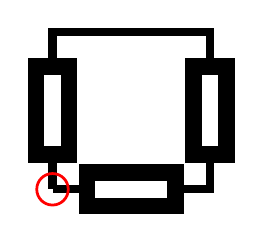
\begin{tikzpicture}[line width=3pt,european]
	\draw (0,0) to[R]++(2,0)to[R]++(0,2)
		--++(-2,0)to[R]++(0,-2);
	\draw[red,line width=1pt] circle(2mm);
	\end{tikzpicture}
\end{LTXexample}
To correct the line ending, there are support shapes to fill this rectangle. They can be used like the support shapes(*,o,d) using a dot (.) on one or both ends of a component(have a look at the last resistor in this example:
\begin{LTXexample}[varwidth=true]
	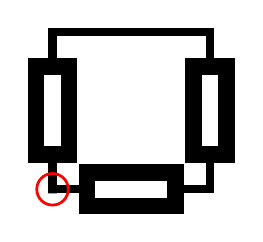
\begin{tikzpicture}[line width=3pt,european]
	\draw (0,0) to[R]++(2,0)to[R]++(0,2)
		--++(-2,0)to[R,-.]++(0,-2);
	\draw[red,line width=1pt] circle(2mm);
	\end{tikzpicture}
\end{LTXexample}


\section{Not only bipoles}
Since only bipoles (but see section~\ref{sec:transasbip}) can be placed "along a line", components with more than two terminals are placed as nodes:
\begin{LTXexample}[varwidth=true]
\begin{circuitikz}
\draw (0,0) node[npn](npn)  at (0,0) {};
\draw (npn.C) --++(0,0.5) node[vcc]{+5\,\textnormal{V}};
\draw (npn.E) --++(0,-0.5) node[vee]{-5\,\textnormal{V}};
\end{circuitikz}
\end{LTXexample}

\subsection{Anchors}

In order to allow connections with other components, all components define anchors. 

\subsubsection{Logical ports} All logical ports, except \textsc{not}, have two inputs and one output. They are called respectively \texttt{in 1}, \texttt{in 2}, \texttt{out}:

\begin{LTXexample}[varwidth=true]
\begin{circuitikz} \draw 
  (0,0) node[and port] (myand)  {}
  (myand.in 1) node[anchor=east] {1}
  (myand.in 2) node[anchor=east] {2}
  (myand.out) node[anchor=west] {3}
;\end{circuitikz}
\end{LTXexample}

\begin{LTXexample}[varwidth=true]
\begin{circuitikz} \draw 
  (0,2) node[and port] (myand1)  {}
  (0,0) node[and port] (myand2)  {}
  (2,1) node[xnor port] (myxnor)  {}
  (myand1.out) -| (myxnor.in 1)
  (myand2.out) -| (myxnor.in 2)
;\end{circuitikz}
\end{LTXexample}

In the case of \textsc{not}, there are only \texttt{in} and \texttt{out} (although for compatibility reasons \texttt{in 1} is still defined and equal to \texttt{in}):

\begin{LTXexample}[varwidth=true]
\begin{circuitikz} \draw 
  (1,0) node[not port] (not1)  {}
  (3,0) node[not port] (not2)  {}
  (0,0) -- (not1.in) 
  (not2.in) -- (not1.out) 
  ++(0,-1) node[ground] {} to[C] (not1.out) 
  (not2.out) -| (4,1) -| (0,0)
;\end{circuitikz}
\end{LTXexample}

\subsubsection{Transistors} For \textsc{nmos}, \textsc{pmos}, \textsc{nfet}, \textsc{nigfete}, \textsc{nigfetd}, \textsc{pfet}, \textsc{pigfete}, and \textsc{pigfetd}  transistors  one has \texttt{base}, \texttt{gate}, \texttt{source} and \texttt{drain} anchors (which can be abbreviated with \texttt{B}, \texttt{G}, \texttt{S} and \texttt{D}):

\begin{LTXexample}[varwidth=true]
\begin{circuitikz} \draw 
  (0,0) node[nmos] (mos)  {}
  (mos.gate) node[anchor=east] {G}
  (mos.drain) node[anchor=south] {D}
  (mos.source) node[anchor=north] {S}
;\end{circuitikz}
\end{LTXexample}

\begin{LTXexample}[varwidth=true]
\begin{circuitikz} \draw 
  (0,0) node[pigfete] (pigfete)  {}
  (pigfete.G) node[anchor=east] {G}
  (pigfete.D) node[anchor=north] {D}
  (pigfete.S) node[anchor=south] {S}
  (pigfete.bulk) node[anchor=west] {Bulk}
;\end{circuitikz}
\end{LTXexample}

Similarly \textsc{njfet} and \textsc{pjfet} have  \texttt{gate}, \texttt{source} and \texttt{drain} anchors (which can be abbreviated with  \texttt{G}, \texttt{S} and \texttt{D}):

\begin{LTXexample}[varwidth=true]
\begin{circuitikz} \draw 
  (0,0) node[pjfet] (pjfet)  {}
  (pjfet.G) node[anchor=east] {G}
  (pjfet.D) node[anchor=north] {D}
  (pjfet.S) node[anchor=south] {S}
;\end{circuitikz}
\end{LTXexample}

For \textsc{npn}, \textsc{pnp}, \textsc{nigbt}, and \textsc{pigbt} transistors the anchors are  \texttt{base}, \texttt{emitter} and \texttt{collector} anchors (which can be abbreviated with \texttt{B}, \texttt{E} and \texttt{C}):

\begin{LTXexample}[varwidth=true]
\begin{circuitikz} \draw 
  (0,0) node[npn] (npn)  {}
  (npn.base) node[anchor=east] {B}
  (npn.collector) node[anchor=south] {C}
  (npn.emitter) node[anchor=north] {E}
;\end{circuitikz}
\end{LTXexample}

\begin{LTXexample}[varwidth=true]
\begin{circuitikz} \draw 
  (0,0) node[pigbt] (pigbt)  {}
  (pigbt.B) node[anchor=east] {B}
  (pigbt.C) node[anchor=north] {C}
  (pigbt.E) node[anchor=south] {E}
;\end{circuitikz}
\end{LTXexample}

Here is one composite example (please notice that the \texttt{xscale=-1} style would also reflect the label of the transistors, so here a new node is added and its text is used, instead of that of \texttt{pnp1}):

\begin{LTXexample}[varwidth=true]
\begin{circuitikz} \draw 
  (0,0) node[pnp] (pnp2) {2}
  (pnp2.B) node[pnp, xscale=-1, anchor=B] (pnp1) {}
    (pnp1) node {1}
  (pnp1.C) node[npn, anchor=C] (npn1) {}
  (pnp2.C) node[npn, xscale=-1, anchor=C] (npn2) {}
  (pnp1.E) -- (pnp2.E)  (npn1.E) -- (npn2.E)
  (pnp1.B) node[circ] {} |- (pnp2.C) node[circ] {}
;\end{circuitikz}
\end{LTXexample}

Similarly, transistors and other components can be reflected vertically:
\begin{LTXexample}[varwidth=true]
\begin{circuitikz} \draw 
  (0,0) node[pigfete, yscale=-1] (pigfete)  {}
  (pigfete.bulk) node[anchor=west] {Bulk}
  (pigfete.G) node[anchor=east] {G}
  (pigfete.D) node[anchor=south] {D}
  (pigfete.S) node[anchor=north] {S}
;\end{circuitikz}
\end{LTXexample}

\begin{LTXexample}[varwidth=true]
   \begin{circuitikz}
        \draw (0,2) 
            node[rground, yscale=-1] {} 
        to[R=$R_1$] (0,0) 
            node[sground] {};
    \end{circuitikz} 
\end{LTXexample}

\subsubsection{Other tripoles} When inserting a thrystor, a triac or a potentiometer, one needs to refer to the third node--gate (\texttt{gate} or \texttt{G}) for the former two; wiper (\texttt{wiper} or \texttt{W}) for the latter one. This is done by giving a name to the bipole:
\label{bipole-naming}
\begin{LTXexample}[varwidth=true]
\begin{circuitikz} \draw 
  (0,0) to[Tr, n=TRI] (2,0) 
        to[pR, n=POT] (4,0);
  \draw[dashed] (TRI.G) -| (POT.wiper) 
;\end{circuitikz}
\end{LTXexample}

As for the switches:
\begin{LTXexample}[varwidth=true]
\begin{circuitikz} \draw 
  (0,0) node[spdt] (Sw) {}
  (Sw.in) node[left] {in}
  (Sw.out 1) node[right] {out 1}
  (Sw.out 2) node[right] {out 2}
;\end{circuitikz}
\end{LTXexample}
\begin{LTXexample}[varwidth=true]
\begin{circuitikz} \draw 
 (0,0) to[C] (1,0) to[toggle switch , n=Sw] (2.5,0) 
   -- (2.5,-1) to[battery1] (1.5,-1) to[R] (0,-1) -| (0,0)
  (Sw.out 2) -| (2.5, 1) to[R] (0,1) -- (0,0)
;\end{circuitikz}
\end{LTXexample}

The ports of the mixer and adder can be addressed with numbers or \texttt{west}/\texttt{south}/\texttt{east}/\texttt{north}:
\begin{LTXexample}[varwidth=true]
\begin{circuitikz} \draw 
  (0,0) node[mixer] (mix) {}
  (mix.1) node[left] {1}
  (mix.2) node[below] {2}
  (mix.3) node[right] {3}
  (mix.4) node[above] {4}
;\end{circuitikz}
\end{LTXexample}

The Wilkinson divider has:
\begin{LTXexample}[varwidth=true]
\begin{circuitikz} \draw
  (0,0) node[wilkinson] (w) {\SI{3}{dB}}
  (w.in) to[short,-o] ++(-0.5,0)
  (w.out1) to[short,-o] ++(0.5,0)
  (w.out2) to[short,-o] ++(0.5,0)
  (w.in) node[below left] {\texttt{in}}
  (w.out1) node[below right] {\texttt{out1}}
  (w.out2) node[above right] {\texttt{out2}}
  ;
\end{circuitikz}
\end{LTXexample}

\subsubsection{Operational amplifier} The op amp defines the inverting input (\texttt{-}), the non-inverting input (\texttt{+}) and the output (\texttt{out}) anchors:

\begin{LTXexample}[varwidth=true]
\begin{circuitikz} \draw 
  (0,0) node[op amp] (opamp) {}
  (opamp.+) node[left] {$v_+$}
  (opamp.-) node[left] {$v_-$}
  (opamp.out) node[right] {$v_o$}
  (opamp.up) --++(0,0.5) node[vcc]{5\,\textnormal{V}}
  (opamp.down) --++(0,-0.5) node[vee]{-5\,\textnormal{V}}
;\end{circuitikz}
\end{LTXexample}

There are also two more anchors defined, \texttt{up} and \texttt{down}, for the power supplies:
\begin{LTXexample}[varwidth=true]
\begin{circuitikz} \draw 
  (0,0) node[op amp] (opamp) {}
  (opamp.+) node[left] {$v_+$}
  (opamp.-) node[left] {$v_-$}
  (opamp.out) node[right] {$v_o$}
  (opamp.down) node[ground] {}
  (opamp.up) ++ (0,.5) node[above] {\SI{12}{\volt}} 
     -- (opamp.up)
;\end{circuitikz}
\end{LTXexample}

The fully differential op amp defines two outputs:
\begin{LTXexample}[varwidth=true]
\begin{circuitikz} \draw 
  (0,0) node[fd op amp] (opamp) {}
  (opamp.+) node[left] {$v_+$}
  (opamp.-) node[left] {$v_-$}
  (opamp.out +) node[right] {out +}
  (opamp.out -) node[right] {out -}
  (opamp.down) node[ground] {}
;\end{circuitikz}
\end{LTXexample}

\subsubsection{Double bipoles} All the (few, actually) double bipoles/quadrupoles have
the four anchors, two for each port. The first port, to the left, is port \texttt{A}, having the anchors \texttt{A1} (up) and \texttt{A2} (down); same for port \texttt{B}. They also expose the \texttt{base} anchor, for labelling:

\begin{LTXexample}[varwidth=true]
\begin{circuitikz} \draw 
  (0,0) node[transformer] (T) {}
  (T.A1) node[anchor=east] {A1}
  (T.A2) node[anchor=east] {A2}
  (T.B1) node[anchor=west] {B1}
  (T.B2) node[anchor=west] {B2}
  (T.base) node{K}
;\end{circuitikz}
\end{LTXexample}

\begin{LTXexample}[varwidth=true]
\begin{circuitikz} \draw 
  (0,0) node[gyrator] (G) {}
  (G.A1) node[anchor=east] {A1}
  (G.A2) node[anchor=east] {A2}
  (G.B1) node[anchor=west] {B1}
  (G.B2) node[anchor=west] {B2}
  (G.base) node{K}
;\end{circuitikz}
\end{LTXexample}

However:
\begin{LTXexample}[varwidth=true]
\begin{circuitikz} \draw
  (0,0) node[coupler] (c) {\SI{10}{dB}}
  (c.1) to[short,-o] ++(-0.5,0)
  (c.2) to[short,-o] ++(0.5,0)
  (c.3) to[short,-o] ++(0.5,0)
  (c.4) to[short,-o] ++(-0.5,0)
  (c.1) node[below left] {\texttt{1}}
  (c.2) node[below right] {\texttt{2}}
  (c.3) node[above right] {\texttt{3}}
  (c.4) node[above left] {\texttt{4}}
  ;
\end{circuitikz}
\end{LTXexample}
		
\begin{LTXexample}[varwidth=true]
\begin{circuitikz} \draw
  (0,0) node[coupler2] (c) {\SI{3}{dB}}
  (c.1) to[short,-o] ++(-0.5,0)
  (c.2) to[short,-o] ++(0.5,0)
  (c.3) to[short,-o] ++(0.5,0)
  (c.4) to[short,-o] ++(-0.5,0)
  (c.1) node[below left] {\texttt{1}}
  (c.2) node[below right] {\texttt{2}}
  (c.3) node[above right] {\texttt{3}}
  (c.4) node[above left] {\texttt{4}}
  ;
\end{circuitikz}
\end{LTXexample}


\subsection{Input arrows}
\subsubsection*{Two ports}
With the option \texttt{>} you can draw an arrow to the input of the block diagram symbols.
\begin{LTXexample}[varwidth=true]
\begin{circuitikz} \draw
  (0,0) to[short,o-] ++(0.3,0)
  to[lowpass,>] ++(2,0)
  to[adc,>] ++(2,0)
  to[short,-o] ++(0.3,0);
\end{circuitikz}
\end{LTXexample}


\subsubsection*{Multi ports}
Since inputs and outputs can vary, input arrows can be placed as nodes. Note that you have to rotate the arrow on your own:
\begin{LTXexample}[varwidth=true]
\begin{circuitikz} \draw
  (0,0) node[mixer] (m) {}
  (m.1) to[short,-o] ++(-1,0)
  (m.2) to[short,-o] ++(0,-1)
  (m.3) to[short,-o] ++(1,0)
  (m.1) node[inputarrow] {}
  (m.2) node[inputarrow,rotate=90] {};
\end{circuitikz}
\end{LTXexample}


\subsection{Labels and custom twoport boxes}
Some twoports have the option to place a normal label (\texttt{l=}) and a inner label (\texttt{t=}).
\begin{LTXexample}[varwidth=true]
\begin{circuitikz}
  \ctikzset{bipoles/amp/width=0.9}
  \draw (0,0) to[amp,t=LNA,l_=$F{=}0.9\,$dB,o-o] ++(3,0);
\end{circuitikz}
\end{LTXexample}


\subsection{Box option}
Some devices have the possibility to add a box around them. The inner symbol scales down to fit inside the box.
\begin{LTXexample}[varwidth=true]
\begin{circuitikz} \draw
  (0,0) node[mixer,box,anchor=east] (m) {}
    to[amp,box,>,-o] ++(2.5,0)
  (m.west) node[inputarrow] {} to[short,-o] ++(-0.8,0)
  (m.south) node[inputarrow,rotate=90] {} --
    ++(0,-0.7) node[oscillator,box,anchor=north] {};
\end{circuitikz}
\end{LTXexample}


\subsection{Dash optional parts}
To show that a device is optional, you can dash it. The inner symbol will be kept with solid lines.
\begin{LTXexample}[varwidth=true]
\begin{circuitikz}
  \draw (0,0) to[amp,l=\SI{10}{dB}] ++(2.5,0);
  \draw[dashed] (2.5,0) to[lowpass,l=opt.] ++(2.5,0);
\end{circuitikz}
\end{LTXexample}

\subsection{Transistor paths}\label{sec:transasbip}

For syntactical convenience transistors can be placed using the normal path notation used for bipoles. The transitor type can be specified by  simply adding a ``T'' (for transistor) in front of the node name of the transistor. It will be placed with the base/gate orthogonal to the direction of the path:
\begin{LTXexample}[varwidth=true]
\begin{circuitikz} \draw
  (0,0) node[njfet] {1}
  (-1,2) to[Tnjfet=2] (1,2) 
    to[Tnjfet=3, mirror] (3,2);
;\end{circuitikz}
\end{LTXexample}

Access to the gate and/or base nodes can be gained by naming the transistors with the \texttt{n} or \texttt{name} path style:
\begin{LTXexample}[varwidth=true]
\begin{circuitikz} \draw[yscale=1.1, xscale=.8]
  (2,4.5) -- (0,4.5) to[Tpmos, n=p1] (0,3) 
     to[Tnmos, n=n1] (0,1.5) 
     to[Tnmos, n=n2] (0,0) node[ground] {}
  (2,4.5) to[Tpmos,n=p2] (2,3) to[short, -*] (0,3)
  (p1.G) -- (n1.G) to[short, *-o] ($(n1.G)+(3,0)$)
  (n2.G) ++(2,0) node[circ] {} -| (p2.G)
  (n2.G) to[short, -o] ($(n2.G)+(3,0)$)
  (0,3) to[short, -o] (-1,3)
;\end{circuitikz}
\end{LTXexample}

The \texttt{name} property is available also for bipoles, although this is useful mostly for triac, potentiometer and thyristor (see~\ref{sec:othertrip}).

\section{Customization}

\subsection{Parameters}

Pretty much all Circui\TikZ\ relies heavily on \texttt{pgfkeys} for value handling and configuration. Indeed, at the beginning of \texttt{circuitikz.sty} a series of key definitions can be found that modify all the graphical characteristics of the package.

All can be varied using the \verb!\ctikzset! command, anywhere in the code.

\paragraph{Shape of the components} (on a per-component-class basis)
\begin{LTXexample}[varwidth=true]
\tikz \draw (0,0) to[R=1<\ohm>] (2,0); \par
\ctikzset{bipoles/resistor/height=.6}
\tikz \draw (0,0) to[R=1<\ohm>] (2,0);
\end{LTXexample}

\begin{LTXexample}[varwidth=true]
\tikz \draw (0,0) node[nand port] {}; \par
\ctikzset{tripoles/american nand port/input height=.2}
\ctikzset{tripoles/american nand port/port width=.2}
\tikz \draw (0,0) node[nand port] {};
\end{LTXexample}

\paragraph{Thickness of the lines} (globally)
\begin{LTXexample}[varwidth=true]
\tikz \draw (0,0) to[C=1<\farad>] (2,0); \par
\ctikzset{bipoles/thickness=1}
\tikz \draw (0,0) to[C=1<\farad>] (2,0);
\end{LTXexample}


\paragraph{Global properties} Of voltage and current
\begin{LTXexample}[varwidth=true]
\tikz \draw (0,0) to[R, v=1<\volt>] (2,0); \par
\ctikzset{voltage/distance from node=.1}
\tikz \draw (0,0) to[R, v=1<\volt>] (2,0);
\end{LTXexample}

\begin{LTXexample}[varwidth=true]
\tikz \draw (0,0) to[C, i=$\imath$] (2,0); \par
\ctikzset{current/distance = .2}
\tikz \draw (0,0) to[C, i=$\imath$] (2,0);
\end{LTXexample}

\noindent However, you can override the properties \verb!voltage/distance from node!\footnote{That is, how distant from the initial and final points of the path the arrow starts and ends.}, \verb!voltage/bump b!\footnote{Controlling how high the bump of the arrow is --- how curved it is.} and \verb!voltage/european label distance!\footnote{Controlling how distant from the bipole the voltage label will be.} on a per-component basis, in order to fine-tune the voltages:

\begin{LTXexample}[varwidth=true]
\tikz \draw (0,0) to[R, v=1<\volt>] (1.5,0) 
       to[C, v=2<\volt>] (3,0); \par
\ctikzset{bipoles/capacitor/voltage/%
     distance from node/.initial=.7}
\tikz \draw (0,0) to[R, v=1<\volt>] (1.5,0)
       to[C, v=2<\volt>] (3,0); \par
\end{LTXexample}

\noindent Admittedly, not all graphical properties have understandable names, but for the time it will have to do:
\begin{LTXexample}[varwidth=true]
\tikz \draw (0,0) node[xnor port] {};
\ctikzset{tripoles/american xnor port/aaa=.2}
\ctikzset{tripoles/american xnor port/bbb=.6} 
\tikz \draw (0,0) node[xnor port] {};
\end{LTXexample}

\subsection{Components size}
Perhaps the most important parameter is \verb!\circuitikzbasekey/bipoles/length!, which 
can be interpreted as the length of a resistor (including reasonable connections): all other lenghts are relative to this value. For instance:

\begin{LTXexample}[pos=t,varwidth=true]
\ctikzset{bipoles/length=1.4cm} 
\begin{circuitikz}[scale=1.2]\draw
  (0,0) node[anchor=east] {B}
        to[short, o-*] (1,0)
        to[R=20<\ohm>, *-*] (1,2)
        to[R=10<\ohm>, v=$v_x$] (3,2) -- (4,2)
        to[cI=$\frac{\si{\siemens}}{5} v_x$, *-*] (4,0) -- (3,0)
        to[R=5<\ohm>, *-*] (3,2)
  (3,0) -- (1,0)
  (1,2) to[short, -o] (0,2) node[anchor=east]{A}  
;\end{circuitikz}
\end{LTXexample}

\begin{LTXexample}[pos=t,varwidth=true]
\ctikzset{bipoles/length=.8cm} 
\begin{circuitikz}[scale=1.2]\draw
  (0,0) node[anchor=east] {B}
        to[short, o-*] (1,0)
        to[R=20<\ohm>, *-*] (1,2)
        to[R=10<\ohm>, v=$v_x$] (3,2) -- (4,2)
        to[cI=$\frac{\siemens}{5} v_x$, *-*] (4,0) -- (3,0)
        to[R=5<\ohm>, *-*] (3,2)
  (3,0) -- (1,0)
  (1,2) to[short, -o] (0,2) node[anchor=east]{A}  
;\end{circuitikz}
\end{LTXexample}

\subsection{Colors}

The color of the components is stored in the key \verb!\circuitikzbasekey/color!. Circui\TikZ\ tries to follow the color set in \TikZ, although sometimes it fails. If you change color in the picture, please do not use just the color name as a style, like \verb![red]!, but rather assign the style \verb![color=red]!.

Compare for instance
\begin{LTXexample}[varwidth=true]
\begin{circuitikz} \draw[red]
  (0,2) node[and port] (myand1)  {}
  (0,0) node[and port] (myand2)  {}
  (2,1) node[xnor port] (myxnor)  {}
  (myand1.out) -| (myxnor.in 1)
  (myand2.out) -| (myxnor.in 2)
;\end{circuitikz}
\end{LTXexample}

and

\begin{LTXexample}[varwidth=true]
\begin{circuitikz} \draw[color=red]
  (0,2) node[and port] (myand1)  {}
  (0,0) node[and port] (myand2)  {}
  (2,1) node[xnor port] (myxnor)  {}
  (myand1.out) -| (myxnor.in 1)
  (myand2.out) -| (myxnor.in 2)
;\end{circuitikz}
\end{LTXexample}

One can of course change the color \emph{in medias res}:
\begin{LTXexample}[pos=t, varwidth=true]
\begin{circuitikz} \draw 
  (0,0) node[pnp, color=blue] (pnp2) {}
  (pnp2.B) node[pnp, xscale=-1, anchor=B, color=brown] (pnp1) {}
  (pnp1.C) node[npn, anchor=C, color=green] (npn1) {}
  (pnp2.C) node[npn, xscale=-1, anchor=C, color=magenta] (npn2) {}
  (pnp1.E) -- (pnp2.E)  (npn1.E) -- (npn2.E)
  (pnp1.B) node[circ] {} |- (pnp2.C) node[circ] {}
;\end{circuitikz}
\end{LTXexample}

The all-in-one stream of bipoles poses some challanges, as only the actual body of the bipole, and not the connecting lines, will be rendered in the specified color. Also, please notice the curly braces around the \texttt{to}:
\begin{LTXexample}[varwidth=true]
\begin{circuitikz} \draw 
  (0,0) to[V=1<\volt>] (0,2)
      { to[R=1<\ohm>, color=red] (2,2) }
        to[C=1<\farad>] (2,0) -- (0,0)
;\end{circuitikz}
\end{LTXexample}

Which, for some bipoles, can be frustrating:
\begin{LTXexample}[varwidth=true]
\begin{circuitikz} \draw 
  (0,0){to[V=1<\volt>, color=red] (0,2) }
        to[R=1<\ohm>] (2,2) 
        to[C=1<\farad>] (2,0) -- (0,0)
;\end{circuitikz}
\end{LTXexample}

The only way out is to specify different paths:
\begin{LTXexample}[varwidth=true]
\begin{circuitikz} \draw[color=red]
  (0,0) to[V=1<\volt>, color=red] (0,2);
  \draw (0,2) to[R=1<\ohm>] (2,2) 
        to[C=1<\farad>] (2,0) -- (0,0)
;\end{circuitikz}
\end{LTXexample}

And yes: this is a bug and \emph{not} a feature\ldots

\section{FAQ}

\noindent Q: When using \verb!\tikzexternalize! I get the following error:
\begin{verbatim}
 ! Emergency stop.
\end{verbatim}

\noindent A: The \TikZ\ manual states:
\begin{quotation}
Furthermore, the library assumes that all \LaTeX\ pictures are ended
    with \verb!\end{tikzpicture}!.
\end{quotation}

Just substitute every occurrence of the environment \verb!circuitikz! with \verb!tikzpicture!. They are actually pretty much the same.

\bigskip

\noindent Q: How do I draw the voltage between two nodes?

\noindent A: Between any two nodes there is an open circuit!
\begin{LTXexample}[varwidth=true]
\begin{circuitikz} \draw
  node[ocirc] (A) at (0,0) {}
  node[ocirc] (B) at (2,1) {}
  (A) to[open, v=$v$] (B)
;\end{circuitikz}
\end{LTXexample}

\bigskip

\noindent Q: I cannot write \verb!to[R = $R_1=12V$]! nor \verb!to[ospst = open, 3s]!: I get errors.

\noindent A: It is a limitation of the \TikZ\ parser. Use \verb!to[R = $R_1{=}12V$]! and \verb!to[ospst = open{,} 3s]! instead.


\section{Examples}
\begin{LTXexample}[pos=t,varwidth=true]
\begin{circuitikz}[scale=1.4]\draw
  (0,0) to[C, l=10<\micro\farad>] (0,2) -- (0,3)
        to[R, l=2.2<\kilo\ohm>] (4,3) -- (4,2)
        to[L, l=12<\milli\henry>, i=$i_1$,v=b] (4,0) -- (0,0)
  (4,2) { to[D*, *-*, color=red] (2,0) }
  (0,2) to[R, l=1<\kilo\ohm>, *-] (2,2) 
        to[cV, i=1,v=$\SI{.3}{\kilo\ohm} i_1$] (4,2)
  (2,0) to[I, i=1<\milli\ampere>, -*] (2,2) 
;\end{circuitikz}
\end{LTXexample}

\begin{LTXexample}[pos=t,varwidth=true]
\begin{circuitikz}[scale=1.2]\draw
  (0,0) node[ground] {}
        to[V=$e(t)$, *-*] (0,2) to[C=4<\nano\farad>] (2,2)
        to[R, l_=.25<\kilo\ohm>, *-*] (2,0)
  (2,2) to[R=1<\kilo\ohm>] (4,2)
        to[C, l_=2<\nano\farad>, *-*] (4,0)
  (5,0) to[I, i_=$a(t)$, -*] (5,2) -- (4,2)
  (0,0) -- (5,0)
  (0,2) -- (0,3) to[L, l=2<\milli\henry>] (5,3) -- (5,2)
 
 {[anchor=south east] (0,2) node {1} (2,2) node {2} (4,2) node {3}}
;\end{circuitikz}
\end{LTXexample}

\begin{LTXexample}[pos=t,varwidth=true]
\begin{circuitikz}[scale=1.2]\draw
  (0,0) node[anchor=east] {B}
        to[short, o-*] (1,0)
        to[R=20<\ohm>, *-*] (1,2)
        to[R=10<\ohm>, v=$v_x$] (3,2) -- (4,2)
        to[cI=$\frac{\siemens}{5} v_x$, *-*] (4,0) -- (3,0)
        to[R=5<\ohm>, *-*] (3,2)
  (3,0) -- (1,0)
  (1,2) to[short, -o] (0,2) node[anchor=east]{A}  
;\end{circuitikz}
\end{LTXexample}
 
\begin{LTXexample}[pos=t,varwidth=true]
\begin{circuitikz}[scale=1]\draw
	(0,0) node[transformer] (T) {}
	(T.B2) to[pD] ($(T.B2)+(2,0)$) -| (3.5, -1)
	(T.B1) to[pD] ($(T.B1)+(2,0)$)  -| (3.5, -1)
;\end{circuitikz}
\end{LTXexample}


\begin{LTXexample}[pos=t,varwidth=true]
\begin{circuitikz}[scale=1]\draw
	(5,.5) node [op amp] (opamp) {}
	(0,0) node [left] {$U_{we}$} to [R, l=$R_d$, o-*] (2,0)
	to [R, l=$R_d$, *-*] (opamp.+)
	to [C, l_=$C_{d2}$, *-] ($(opamp.+)+(0,-2)$) node [ground] {}
	(opamp.out) |- (3.5,2) to [C, l_=$C_{d1}$, *-] (2,2) to [short] (2,0)
	(opamp.-) -| (3.5,2)
	(opamp.out) to [short, *-o] (7,.5) node [right] {$U_{wy}$}
;\end{circuitikz}
\end{LTXexample}
 
\begin{LTXexample}[pos=t,varwidth=true]
\begin{circuitikz}[scale=1.2, american]\draw
  (0,2) to[I=1<\milli\ampere>] (2,2)
        to[R, l_=2<\kilo\ohm>, *-*] (0,0)
        to[R, l_=2<\kilo\ohm>] (2,0)
        to[V, v_=2<\volt>] (2,2)
        to[cspst, l=$t_0$] (4,2) -- (4,1.5)
        to [generic, i=$i_1$, v=$v_1$] (4,-.5) -- (4,-1.5)
  (0,2) -- (0,-1.5) to[V, v_=4<\volt>] (2,-1.5)
        to [R, l=1<\kilo\ohm>] (4,-1.5);

   \begin{scope}[xshift=6.5cm, yshift=.5cm]
    \draw [->] (-2,0) -- (2.5,0) node[anchor=west] {$v_1/\volt$};
    \draw [->] (0,-2) -- (0,2) node[anchor=west] {$i_1/\SI{}{\milli\ampere}$} ;
    \draw (-1,0) node[anchor=north] {-2} (1,0) node[anchor=south] {2}
          (0,1) node[anchor=west] {4} (0,-1) node[anchor=east] {-4} 
          (2,0) node[anchor=north west] {4}
          (-1.5,0) node[anchor=south east] {-3};
    \draw [thick] (-2,-1) -- (-1,1) -- (1,-1) -- (2,0) -- (2.5,.5);
    \draw [dotted] (-1,1) -- (-1,0) (1,-1) -- (1,0) 
          (-1,1) -- (0,1) (1,-1) -- (0,-1);
   \end{scope}  
\end{circuitikz}
\end{LTXexample}

\begin{LTXexample}[pos=t,varwidth=true]
	\begin{circuitikz}[scale=1]
		\ctikzset{bipoles/detector/width=.35}
		\ctikzset{quadpoles/coupler/width=1}
		\ctikzset{quadpoles/coupler/height=1}
		\ctikzset{tripoles/wilkinson/width=1}
		\ctikzset{tripoles/wilkinson/height=1}
		%\draw[help lines,red,thin,dotted] (0,-5) grid (5,5);
		\draw
		(-2,0) node[wilkinson](w1){}
		(2,0) node[coupler] (c1) {}
		(0,2) node[coupler,rotate=90] (c2) {}
		(0,-2) node[coupler,rotate=90] (c3) {}
		(w1.out1) .. controls ++(0.8,0) and ++(0,0.8) .. (c3.3)
		(w1.out2) .. controls ++(0.8,0) and ++(0,-0.8) .. (c2.4)
		(c1.1) .. controls ++(-0.8,0) and ++(0,0.8) .. (c3.2)
		(c1.4) .. controls ++(-0.8,0) and ++(0,-0.8) .. (c2.1)
		(w1.in) to[short,-o] ++(-1,0)
		(w1.in) node[left=30] {LO}
		(c1.2) node[match,yscale=1] {}
		(c1.3) to[short,-o] ++(1,0)
		(c1.3) node[right=30] {RF}
		(c2.3) to[detector,-o] ++(0,1.5)
		(c2.2) to[detector,-o] ++(0,1.5)
		(c3.1) to[detector,-o] ++(0,-1.5)
		(c3.4) to[detector,-o] ++(0,-1.5)
		;
	\end{circuitikz}
\end{LTXexample}


\begin{tabular}{l}\label{ex:compatibility}
	\fbox{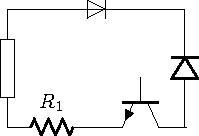
\includegraphics{compatibility.pdf}}
	\\
	\begin{lstlisting}
\documentclass{standalone}

\usepackage{tikz}
\usetikzlibrary{circuits.ee.IEC}
\usetikzlibrary{positioning}

\usepackage[compatibility]{circuitikz}
\ctikzset{bipoles/length=.9cm}

\begin{document}
 \begin{tikzpicture}[circuit ee IEC]
  \draw (0,0) to [resistor={name=R}] (0,2)
	to[diode={name=D}] (3,2);
  \draw (0,0) to[*R=$R_1$] (1.5,0) to[*Tnpn] (3,0)
    to[*D](3,2);
 \end{tikzpicture}
\end{document}
	\end{lstlisting}
\end{tabular}

% % changelog.tex will be updated by makefile from CHANGELOG.md
\section{Changelog}
\IfFileExists{changelog.tex}
{%DO NOT EDIT THIS AUTOMATICALLY GENERATED FILE!!!
The major changes among the different circuitikz versions are listed
here. See \url{https://github.com/mredaelli/circuitikz/commits} for a
full list of changes.

\begin{itemize}
\itemsep1pt\parskip0pt\parsep0pt
\item
  Version 0.5 (2016-04-23)

  \begin{itemize}
  \itemsep1pt\parskip0pt\parsep0pt
  \item
    new option boxed and dashed for hf-symbols
  \item
    new option solderdot to enable/disable solderdot at source port of
    some fets
  \item
    new parts: photovoltaic source, piezo crystal, electrolytic
    capacitor, electromechanical device(motor, generator)
  \item
    corrected voltage and current direction(option to use old behaviour)
  \item
    option to show body diode at fet transistors
  \end{itemize}
\item
  Version 0.4

  \begin{itemize}
  \itemsep1pt\parskip0pt\parsep0pt
  \item
    minor improvements to documentation
  \item
    comply with TDS
  \item
    merge high frequency symbols by Stefan Erhardt
  \item
    added switch (not opening nor closing)
  \item
    added solder dot in some transistors
  \item
    improved ConTeXt compatibility
  \end{itemize}
\item
  Version 0.3.1

  \begin{itemize}
  \itemsep1pt\parskip0pt\parsep0pt
  \item
    different management of color\ldots{}
  \item
    fixed typo in documentation
  \item
    fixed an error in the angle computation in voltage and current
    routines
  \item
    fixed problem with label size when scaling a tikz picture
  \item
    added gas filled surge arrester
  \item
    added compatibility option to work with Tikz's own circuit library
  \item
    fixed infinite in arctan computation
  \end{itemize}
\item
  Version 0.3.0

  \begin{itemize}
  \itemsep1pt\parskip0pt\parsep0pt
  \item
    fixed gate node for a few transistors
  \item
    added mixer
  \item
    added fully differential op amp (by Kristofer M. Monisit)
  \item
    now general settings for the drawing of voltage can be overridden
    for specific components
  \item
    made arrows more homogeneous (either the current one, or latex' bt
    pgf)
  \item
    added the single battery cell
  \item
    added fuse and asymmetric fuse
  \item
    added toggle switch
  \item
    added varistor, photoresistor, thermocouple, push button
  \item
    added thermistor, thermistor ptc, thermistor ptc
  \item
    fixed misalignment of voltage label in vertical bipoles with names
  \item
    added isfet
  \item
    added noiseless, protective, chassis, signal and reference grounds
    (Luigi «Liverpool»)
  \end{itemize}
\item
  Version 0.2.4

  \begin{itemize}
  \itemsep1pt\parskip0pt\parsep0pt
  \item
    added square voltage source (contributed by Alistair Kwan)
  \item
    added buffer and plain amplifier (contributed by Danilo Piazzalunga)
  \item
    added squid and barrier (contributed by Cor Molenaar)
  \item
    added antenna and transmission line symbols contributed by Leonardo
    Azzinnari
  \item
    added the changeover switch spdt (suggestion of Fabio Maria
    Antoniali)
  \item
    rename of context.tex and context.pdf (thanks to Karl Berry)
  \item
    updated the email address
  \item
    in documentation, fixed wrong (non-standard) labelling of the axis
    in an example (thanks to prof. Claudio Beccaria)
  \item
    fixed scaling inconsistencies in quadrupoles\\
  \item
    fixed division by zero error on certain vertical paths
  \item
    introduced options straighlabels, rotatelabels, smartlabels
  \end{itemize}
\item
  Version 0.2.3

  \begin{itemize}
  \itemsep1pt\parskip0pt\parsep0pt
  \item
    fixed compatibility problem with label option from tikz
  \item
    Fixed resizing problem for shape ground
  \item
    Variable capacitor
  \item
    polarized capacitor
  \item
    ConTeXt support (read the manual!)
  \item
    nfet, nigfete, nigfetd, pfet, pigfete, pigfetd (contribution of
    Clemens Helfmeier and Theodor Borsche)
  \item
    njfet, pjfet (contribution of Danilo Piazzalunga)
  \item
    pigbt, nigbt
  \item
    \emph{backward incompatibility} potentiometer is now the standard
    resistor-with-arrow-in-the-middle; the old potentiometer is now
    known as variable resistor (or vR), similarly to variable inductor
    and variable capacitor
  \item
    triac, thyristor, memristor
  \item
    new property ``name'' for bipoles
  \item
    fixed voltage problem for batteries in american voltage mode
  \item
    european logic gates
  \item
    \emph{backward incompatibility} new american standard inductor. Old
    american inductor now called ``cute inductor''
  \item
    \emph{backward incompatibility} transformer now linked with the
    chosen type of inductor, and version with core, too. Similarly for
    variable inductor
  \item
    \emph{backward incompatibility} styles for selecting shape variants
    now end are in the plural to avoid conflict with paths
  \item
    new placing option for some tripoles (mostly transistors)
  \item
    mirror path style
  \end{itemize}
\item
  Version 0.2.2 - 20090520

  \begin{itemize}
  \itemsep1pt\parskip0pt\parsep0pt
  \item
    Added the shape for lamps.
  \item
    Added options \texttt{europeanresistor}, \texttt{europeaninductor},
    \texttt{americanresistor} and \texttt{americaninductor}, with
    corresponding styles.
  \item
    FIXED: error in transistor arrow positioning and direction under
    negative \texttt{xscale} and \texttt{yscale}.
  \end{itemize}
\item
  Version 0.2.1 - 20090503

  \begin{itemize}
  \itemsep1pt\parskip0pt\parsep0pt
  \item
    Op-amps added
  \item
    added options arrowmos and noarrowmos, to add arrows to pmos and
    nmos
  \end{itemize}
\item
  Version 0.2 - 20090417 First public release on CTAN

  \begin{itemize}
  \itemsep1pt\parskip0pt\parsep0pt
  \item
    \emph{Backward incompatibility}: labels ending with
    \texttt{:}\textit{angle} are not parsed for positioning anymore.
  \item
    Full use of \TikZ~keyval features.
  \item
    White background is not filled anymore: now the network can be drawn
    on a background picture as well.
  \item
    Several new components added (logical ports, transistors, double
    bipoles, \ldots).
  \item
    Color support.
  \item
    Integration with \{\ttfamily siunitx\}.
  \item
    Voltage, american style.
  \item
    Better code, perhaps. General cleanup at the very least.
  \end{itemize}
\item
  Version 0.1 - 2007-10-29 First public release
\end{itemize}
}
{The file changelog.tex was not found, run 'make changelog' at toplevel to generate it with pandoc from CHANGELOG.md}

\printindex

\end{document}
